\typeout{(body.tex)}

\begin{frame}
    \titlepage
\end{frame}


\section{briefly: vertices and edges}

\usetikzlibrary{graphs,graphs.standard,graphdrawing,quotes}
\usegdlibrary{force}

\begin{frame}{vertices and edges}
\tikzset{
    graphNode/.style={draw,circle,thick,font=\tt\fontsize{9}{10}\selectfont,minimum width=.6cm,inner sep=0.2mm,text=white,
        alt=<2>{draw=red,ultra thick},alt=<3->{draw=green!50!black}},
    graphEdge/.style={draw,thick,alt=<3>{draw=red,ultra thick},alt=<4->{draw=blue}},
    >=Latex,
    my graph/.style={graphs/nodes={graphNode},graphs/edges={graphEdge},graphs/edge quotes={font=\tt\tiny,auto}},
}

\begin{tikzpicture}
\begin{scope}[my graph]
% https://tex.stackexchange.com/questions/207953/petersen-graph-with-new-tikz-graph-library/208039
  \graph[clockwise, radius=1.5cm] {subgraph C_n [n=5,name=A] };
  \graph[clockwise, radius=0.75cm] {subgraph I_n [n=5,name=B] };

  \foreach \i [evaluate={\j=int(mod(\i+2+4,5)+1)}] in {1,2,3,4,5}{
    \draw[graphEdge] (A \i) -- (B \i);
    \draw[graphEdge] (B \j) -- (B \i);
  }
\end{scope}
\begin{visibleenv}<2->
    \begin{pgfonlayer}{bg}
    \draw[dotted,line width=.5mm,alt=<2>{draw=red!75}{draw=green!50!black},<-] ([xshift=.1cm]A 1.east) -- ++(3cm,0cm) node[right] (vertexOrEdge) {\textbf{vertices} or \textbf{nodes}};
    \draw[dotted,line width=.5mm,alt=<2>{draw=red!75}{draw=green!50!black},<-] ([xshift=.1cm]A 2.north east) -- (vertexOrEdge.west);
    \draw[dotted,line width=.5mm,alt=<2>{draw=red!75}{draw=green!50!black},<-] ([xshift=.1cm]B 1.north east) -- (vertexOrEdge.west);
    \end{pgfonlayer}
\end{visibleenv}

\begin{visibleenv}<3->
    \coordinate (middle1) at ($(A 2)!0.5!(A 3)$);
    \coordinate (middle2) at ($(A 2)!0.7!(B 2)$);
    \coordinate (middle3) at ($(A 3)!0.5!(B 3)$);
    \coordinate (middle4) at ($(B 2)!0.3!(B 4)$);
    \coordinate (edgeLabel) at ([xshift=2cm]middle1);
    \begin{pgfonlayer}{bg}
    \foreach \x in {1,2,3,4} {
        \draw[dotted,line width=.5mm,alt=<3>{draw=red!75}{draw=blue!70!black},<-] ([xshift=.1cm]middle\x) -- (edgeLabel);
    }
    \node[anchor=west] at (edgeLabel) {\textbf{edges}};
    \end{pgfonlayer}
\end{visibleenv}
\begin{visibleenv}<5->
\begin{scope}[my graph,yshift=-4cm]
% https://tex.stackexchange.com/questions/207953/petersen-graph-with-new-tikz-graph-library/208039
  \graph[clockwise, radius=2cm] {subgraph C_n [n=5,name=Ad, ->] };
  \graph[clockwise, radius=1cm] {subgraph I_n [n=5,name=Bd] };

  \foreach \i [evaluate={\j=int(mod(\i+2+4,5)+1)}] in {1,2,3,4,5}{
    \draw[graphEdge,->] (Ad \i) -- (Bd \i);
    \draw[graphEdge,->] (Bd \j) -- (Bd \i);
  }
\end{scope}
\coordinate (dirStart) at ([xshift=-2cm]Ad 1.west);
\coordinate (undirStart) at ([xshift=-2cm]A 1.west);
\draw[very thick,decorate,decoration={brace, mirror}] (dirStart) -- (dirStart |- Ad 4)
    node[midway, left,align=right] {\textbf{directed graph} \\ \textit{or} \\ \textbf{digraph}};
\draw[very thick,decorate,decoration={brace, mirror}] (undirStart) -- (undirStart |- A 4)
    node[midway, left] {\textbf{undirected graph}};
\end{visibleenv}
\end{tikzpicture}
\end{frame}


\section{examples}

\begin{frame}{example graphs}
\begin{itemize}
\item lots of things can be represented as graphs
\end{itemize}
\end{frame}

\begin{frame}{maps}
\begin{tikzpicture}
\node[inner sep=0mm] (the map) {
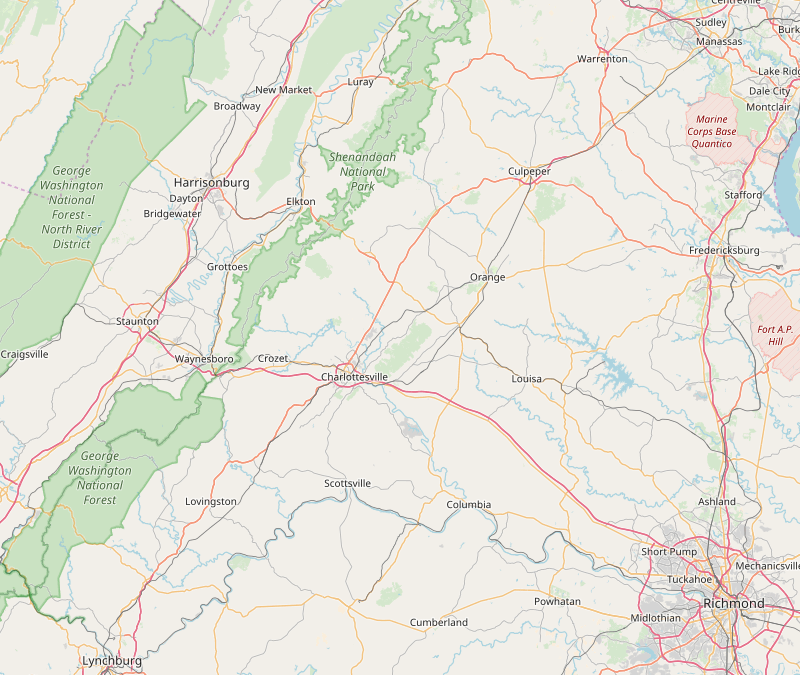
\includegraphics[height=\textheight]{map-example}
};
\node[align=left,right=0cm of the map] {
    nodes: intersections? \\
    edges: roads?
};
\end{tikzpicture}
\imagecredit{image: open street map}
\end{frame}

\begin{frame}{airline routes}
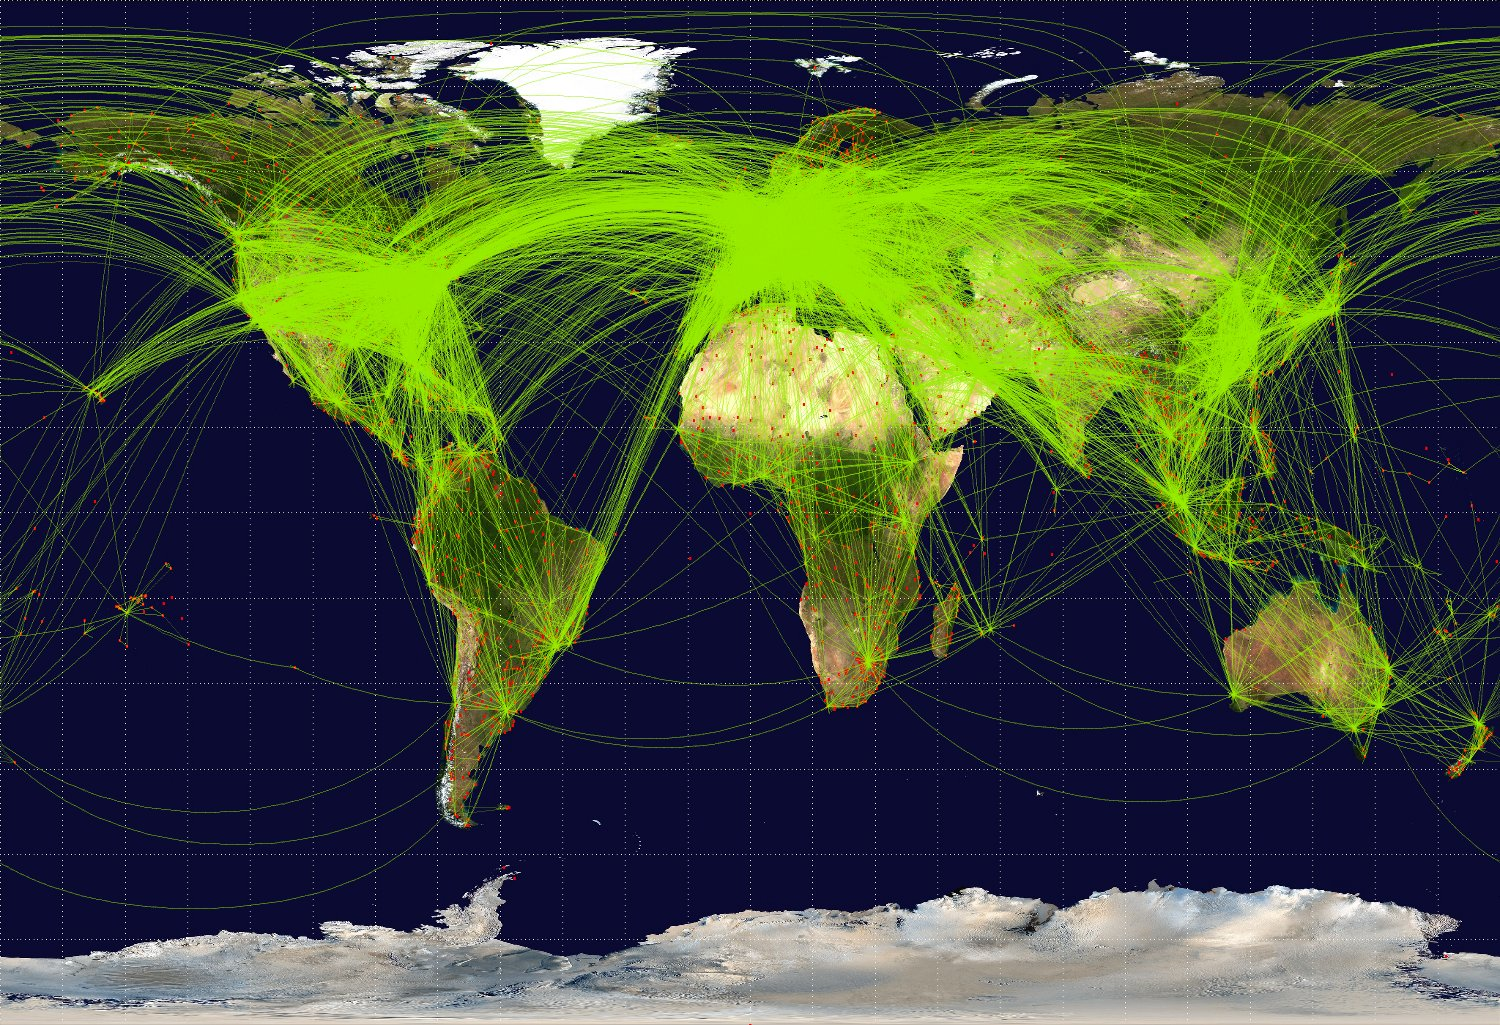
\includegraphics[height=0.9\textheight]{airline-routes-from-openflights}
\imagecredit{image: openflights}
\end{frame}

\begin{frame}{flowcharts}
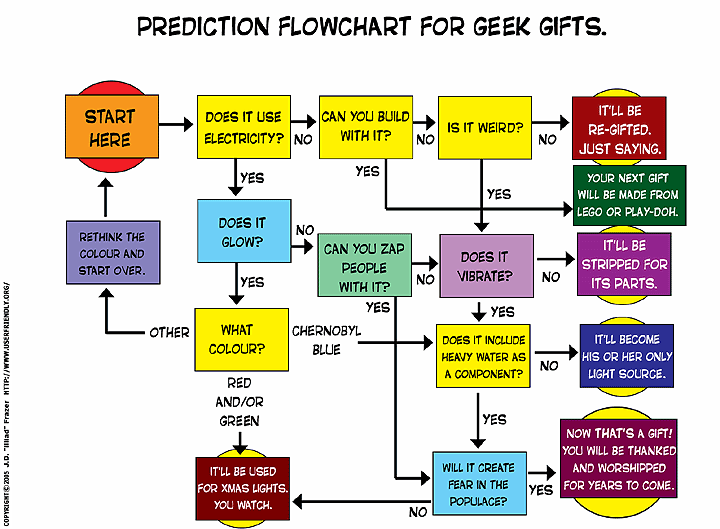
\includegraphics[height=0.9\textheight]{geek-gift-flowchart}
\end{frame}

\begin{frame}[label=preReqTree]{pre-requisite tree}
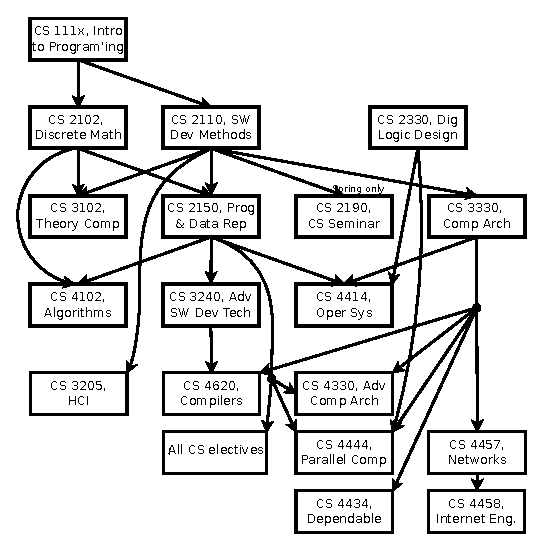
\includegraphics[height=0.9\textheight]{bs-cs-chart}
\end{frame}


\subsection{road networks}

\subsection{airplane routes}

\subsection{flowcharts}

\subsection{prerequisite diagrams}

\subsection{web pages}

% FIXME: missing

\subsection{example: sizes}

% FIXME: missing

\section{formal definitions}

\subsection{vertices, edges}

\begin{frame}{formal definition}
\begin{itemize}
\item graph $G$: $G = (V,E)$
\item $V$: set of vertices (possibly empty)
\item $E$: set of edges --- pairs of vertices (possibly empty)
    \begin{itemize}
    \item directed graph/digraph --- ordered pairs
    \item undirected graph --- unordered pairs
    \end{itemize}
\end{itemize}
\end{frame}


\subsection{paths and path lengths and simple paths}

\begin{frame}{paths, etc.}
\begin{itemize}
\item vertices $v$ and $w$ \textbf{adjacent} iff $(v,w) \in E$
\item \textbf{path}: $v_1, v_2, \ldots v_n$ such that $(v_i, v_{i+1}) \in E$ for $1 \le i \le n$
\item \textbf{length} of path: number of \textbf{edges} in path
\item \textbf{simple path}: path of distinct vertices
\end{itemize}
\end{frame}


\subsection{weights or costs}

\usetikzlibrary{graphs,graphs.standard,graphdrawing,quotes}
\usegdlibrary{force}


\begin{frame}{weighted graphs}
\begin{itemize}
\item some graphs have \textbf{weights} or \textbf{costs} associated with edges
\item example motivation:
    \begin{itemize}
    \item graph representing roads: weight = travel time
    \end{itemize}
\item \textbf{weight} or cost \textbf{of a path} = sum of weights of edges in path
\end{itemize}
\end{frame}

\begin{frame}{weighted graph example}
\begin{tikzpicture}
\tikzset{
    graphNode/.style={draw,thick},
    graphEdge/.style={draw,thick},
    >=Latex,
    my graph/.style={graphs/nodes={graphNode,label={[font=\small,fill=white,fill opacity=0.9]south:\tikzgraphnodetext}},graphs/edges={graphEdge},graphs/edge quotes={font=\small,auto,inner sep=0mm},
        graphs/typeset={},
    },
}
\begin{scope}[my graph,shift={(78,-38)},scale=4]
\graph[no placement] {
    Charlottesville[at={(-78.47,38.03)}],
    Culpeper[at={(-77.99,38.47)}],
    DC[at={(-77.01,38.90)}],
    Richmond[at={(-77.47,37.53)}],
    Fredericksburg[at={(-77.47,38.30)}],

    Charlottesville --["46"] Culpeper --["73"] DC[as={Washington, DC}],
    Charlottesville --["72"] Richmond --["58"] Fredericksburg --["53"] DC,
    Fredericksburg --["35"'] Culpeper,
};
\end{scope}
\end{tikzpicture}
\end{frame}


\subsection{cycles and loops}

% FIXME: # cycles exercise
\usetikzlibrary{graphs,graphs.standard,graphdrawing,quotes}
\usegdlibrary{force}

\begin{frame}{cycles, loops, etc.}
\tikzset{
    my graph node/.style={draw,circle,thick,font=\tt\fontsize{7}{8}\selectfont,minimum width=.3cm,inner sep=0.2mm,text=white},
    my graph edge/.style={draw,thick},
    my graph node hidden/.style={my graph node,opacity=0.5},
    my graph edge hidden/.style={my graph edge,opacity=0.5},
    >=Latex,
    my graph/.style={graphs/nodes={my graph node},graphs/edges={my graph edge},graphs/edge quotes={font=\tt\tiny,auto}},
    my graph hide/.style={graphs/nodes={my graph node hidden},graphs/edges={my graph edge hidden},graphs/edge quotes={font=\tt\tiny,auto}},
    graphs/show cycle/.style={nodes={opacity=1.0,draw=blue!70!black},edges={opacity=1.0,draw=blue!70!black}}
}
\begin{itemize}
\item \textbf{cycle}: path where length $\ge 1$, $v_1=v_n$
\begin{itemize}
\item undirected graph: \ldots and no repeated edges
\end{itemize}
\item \textbf{loop}: $(v,v) \in E$
\end{itemize}
\begin{tikzpicture}[overlay,remember picture]
\begin{scope}[my graph hide]
\graph[spring layout,downsize ratio=0.1,node distance=.5cm] {
    {[show cycle] A -- B -- C -- D -- E -- A},
    X -- A,
    D -- Y,
    C -- R -- Q -- Z -- C,
    A[desired at={([xshift=-3cm,yshift=-4cm]current page.north east)}],
    E[desired at={([xshift=-2.5cm,yshift=-4cm]current page.north east)}],
};

\graph[spring layout,downsize ratio=0.1,node distance=.5cm] {
    {A -- B -- {[show cycle] C} -- D -- E -- A},
    X -- A,
    D -- Y,
    {[show cycle] C -- R -- Q -- Z -- C},
    A[desired at={([xshift=-3cm,yshift=-2cm]current page.north east)}],
    E[desired at={([xshift=-2.5cm,yshift=-2cm]current page.north east)}],
};
\end{scope}
\end{tikzpicture}
\end{frame}


\subsection{a note on alternative definitions}

\begin{frame}{graph terminology is not universal}
\begin{itemize}
\item some sources will use slightly different definitions:
\vspace{.5cm}
\item \textbf{walk} instead of \textbf{path}
\item \textbf{path} instead of \textbf{simple path}
\item \textbf{closed walk} instead of \textbf{cycle}
\item \textbf{cycle} instead of \textbf{cycle that is also a simple path}
\end{itemize}
\end{frame}


\subsection{connectivity, DAGs}

% FIXME: examples
\usetikzlibrary{graphs,graphs.standard,graphdrawing,quotes}
\usegdlibrary{force,circular,routing,layered,trees}


\begin{frame}{connectivity}
\tikzset{
    my graph node/.style={draw,circle,thick,font=\tt\fontsize{7}{8}\selectfont,minimum width=.3cm,inner sep=0.2mm,text=white},
    my graph edge/.style={draw,thick},
    my graph node hidden/.style={my graph node,draw=black!50},
    my graph edge hidden/.style={my graph edge,draw=black!50},
    >=Latex,
    my graph/.style={graphs/nodes={my graph node},graphs/edges={my graph edge},graphs/edge quotes={font=\tt\tiny,auto}},
    my graph hide/.style={graphs/nodes={my graph node hidden},graphs/edges={my graph edge hidden},graphs/edge quotes={font=\tt\tiny,auto}},
    graphs/show cycle/.style={nodes={draw=blue!70!black},edges={opacity=1.0,draw=blue!70!black}},
    graphs/show cycle B/.style={nodes={draw=orange!80!black},edges={opacity=1.0,draw=orange!80!black}},
    show cycle B/.style={draw=orange!80!black,graphs/nodes={draw=orange!80!black},graphs/edges={draw=orange!80!black}},
}
\begin{itemize}
\item \textbf{connected graph}: for all $x, y  \in V$, there exists a path from $x$ to $y$
    \begin{itemize}
    \item N.B: includes 0-length paths
    \end{itemize}
\end{itemize}
\begin{tikzpicture}
\matrix{
\begin{scope}[my graph]
\graph[spring layout] {
    [name=A] A -- B -- C -- D -- B -- D
};
\end{scope}
\node[draw,ultra thick,fit=(A A) (A D) (A C) (A B),label={north:a connected graph}] {};
\&
\begin{scope}[my graph]
\graph[spring layout] {
    [name=B] A -- B -- C,
    D, E -- F
};
\end{scope}
\node[draw,ultra thick,fit=(B A) (B D) (B C) (B B) (B E) (B F),label={north:a non-connected graph}] {};
\\
};
\end{tikzpicture}
\end{frame}

\begin{frame}{in a directed graph\ldots}
\begin{itemize}
\item \textbf{DAG} --- directed acyclic graph
    \begin{itemize}
    \item no cycles
    \end{itemize}
\item \textbf{strongly connected} --- path from every vertex to every other
    \begin{itemize}
    \item implies cycles (or digraph of 0 or 1 nodes)
    \end{itemize}
\item \textbf{weakly connected} --- would be connected as undirected graph
\end{itemize}
\end{frame}

\begin{frame}{strong/weak connected examples}
\begin{tikzpicture}
\tikzset{
    my graph node/.style={draw,circle,thick,font=\tt\fontsize{7}{8}\selectfont,minimum width=.3cm,inner sep=0.2mm},
    my graph edge/.style={draw,thick},
    my graph node hidden/.style={my graph node,draw=black!50},
    my graph edge hidden/.style={my graph edge,draw=black!50},
    >=Latex,
    my graph/.style={graphs/nodes={my graph node},graphs/edges={my graph edge},graphs/edge quotes={font=\tt\tiny,auto}},
    my graph hide/.style={graphs/nodes={my graph node hidden},graphs/edges={my graph edge hidden},graphs/edge quotes={font=\tt\tiny,auto}},
    graphs/show cycle/.style={nodes={draw=blue!70!black},edges={opacity=1.0,draw=blue!70!black}},
    graphs/show cycle B/.style={nodes={draw=orange!80!black},edges={opacity=1.0,draw=orange!80!black}},
    show cycle B/.style={draw=orange!80!black,graphs/nodes={draw=orange!80!black},graphs/edges={draw=orange!80!black}},
    mark graph/.style={draw,very thick},
}
\matrix (scA) {
\node[font=\small,align=center] {a strongly connected graph \\
drawn in two ways};
\\
\node {
\begin{tikzpicture}
\begin{scope}[my graph]
\graph[simple necklace layout] {
    [name=X]
    A -> B -> C -> D -> B -> E -> F ->  A,
    F -> G -> C,
};
\end{scope}
\node[fit=(X A) (X G) (X B) (X D) (X C) (X F),mark graph] {};
\end{tikzpicture}
};
\\
\node {
\begin{tikzpicture}
\begin{scope}[my graph]
\graph[spring layout] {
    [name=Y]
    A -> B -> C -> D -> B -> E -> F ->  A,
    F -> G -> C,
};
\end{scope}
\node[fit=(Y A) (Y G) (Y B) (Y D) (Y C) (Y F),mark graph] {};
\end{tikzpicture}
};
\\
};
\matrix[right=.5cm of scA] (scB) {
\node[font=\small,align=center] {another strongly\\connected graph};
\\
\node {
\begin{tikzpicture}
\begin{scope}[my graph]
\graph[tree layout] {
    [name=Z]
    // [simple necklace layout] { A -> B -> C -> D -> A },
    // [simple necklace layout] { E -> F -> G -> H -> I },
    C -> E,
    I -> C,
};
\end{scope}
\node[fit=(Z A) (Z G) (Z B) (Z D) (Z C) (Z F),mark graph] {};
\end{tikzpicture}
};
\\
};
\matrix[right=.5cm of scB] {
\node[font=\small,align=center] {a weakly connected graph };
\\
\node[mark graph] (weakGraph){
\begin{tikzpicture}
\begin{scope}[my graph]
\graph[spring layout,node distance=1.5cm] {
    [name=W] subgraph K_n [V={a,b,c,d},<->] -> subgraph C_n [V={e,f,g},<->],
};
\end{scope}
\begin{visibleenv}<2>
\node[fit=(W e) (W f) (W g),draw=red,dashed] {};
\node[fit=(W a) (W b) (W c) (W d),draw=red,dashed] {};
\end{visibleenv}
\end{tikzpicture}
};
\\
};
\begin{visibleenv}<2>
\node[below=.5cm of weakGraph,font=\small,red!70!black] {two \textit{strongly connected components}};
\end{visibleenv}
\end{tikzpicture}
\end{frame}


\subsubsection{aside: trees as special case}

\begin{frame}{trees as graphs}
\begin{itemize}
\item trees are connected, acyclic graphs
\begin{itemize}
\item (with a root chosen)
\end{itemize}
\end{itemize}
\end{frame}


\subsection{special graph: complete graph}

\usetikzlibrary{graphs,graphs.standard,graphdrawing,quotes}
\usegdlibrary{force}



\begin{frame}{complete graph}
\tikzset{
    graphNode/.style={draw,circle,thick,font=\tt\fontsize{9}{10}\selectfont,minimum width=.6cm,inner sep=0.2mm,text=white},
    graphEdge/.style={draw,thick},
    >=Latex,
    my graph/.style={graphs/nodes={graphNode},graphs/edges={graphEdge},graphs/edge quotes={font=\tt\tiny,auto}},
}
\begin{itemize}
\item \textbf{complete graph}: graph with edges between every pair of distinct vertices
\end{itemize}
\begin{tikzpicture}
\begin{scope}[my graph]
\graph[clockwise, radius=2.5cm] {subgraph K_n [n=10,name=A] };
\end{scope}
\end{tikzpicture}
\end{frame}


\section{representing graphs}

\subsection{adjacency matrices}

% FIXME: adj. matrix with weights

\usetikzlibrary{graphs,graphs.standard,graphdrawing,quotes}
\usegdlibrary{force}

\begin{frame}{adjacency matrix}
$
A[u][v] = 
    \begin{cases}
        weight  & \text{if } (u, v) \in E \\
        0 & \text{otherwise} \\
    \end{cases}
$
% $

\begin{tikzpicture}
\matrix[tight matrix,
    row 1/.style={nodes={draw=none}},
    column 1/.style={nodes={draw=none}},
    ] (theAdj) {
    ~ \& 1 \& 2 \& 3 \& 4 \\
    1 \& 0 \& 1 \& 1 \& 1 \\
    2 \& 0 \& 0 \& |[{alt=<2>{fill=red!10}}]| 1 \& 0 \\
    3 \& 0 \& 0 \& 0 \& 0 \\
    4 \& |[{alt=<3>{fill=red!10}}]| 1 \& 0 \& 0 \& 0 \\
};
\tikzset{
    graphNode/.style={draw,circle,thick,font=\tt\fontsize{9}{10}\selectfont,minimum width=.6cm,inner sep=0.2mm},
    graphEdge/.style={draw,thick},
    >=Latex,
    my graph/.style={graphs/nodes={graphNode},graphs/edges={graphEdge},graphs/edge quotes={font=\tt\tiny,auto}},
}
\begin{scope}[my graph]
\graph[spring layout] {
    1[desired at={([xshift=2cm]theAdj.east)}] -> 2,
    1 -> 3,
    2 -> 3[> alt=<2>{red,very thick}],
    1 -> 4[> bend left,> alt=<3>{red,very thick}],
    4 -> 1[> bend left],
};
\end{scope}
\end{tikzpicture}
\begin{visibleenv}<4>
\begin{tikzpicture}
\matrix[tight matrix,
    row 1/.style={nodes={draw=none}},
    column 1/.style={nodes={draw=none}},
    ] (theAdj) {
    ~ \& 1 \& 2 \& 3 \& 4 \\
    1 \& 9 \& 17 \& 0 \& 0 \\
    2 \& 0 \& 0 \& 13 \& 0 \\
    3 \& 0 \& 0 \& 0 \& 10 \\
    4 \& 0 \& 16 \& 18 \& 0 \\ 
};
\tikzset{
    graphNode/.style={draw,circle,thick,font=\tt\fontsize{9}{10}\selectfont,minimum width=.6cm,inner sep=0.2mm},
    graphEdge/.style={draw,thick},
    >=Latex,
    my graph/.style={graphs/nodes={graphNode},graphs/edges={graphEdge},graphs/edge quotes={font=\tt\tiny,auto}},
}
\begin{scope}[my graph,node distance=1.5cm]
\graph[spring layout] {
    1[desired at={([xshift=1cm]theAdj.east)}] ->["17",orient=right] 2 ->["13"] 3 ->["10"] -> 4,
    4 ->["16"] 2, 
    4 ->["18"] 3, 
    1 ->[loop above, "9"] 1,
};
\end{scope}
\end{tikzpicture}
\end{visibleenv}
\end{frame}


\subsection{adjacency lists}

\usetikzlibrary{graphs,graphs.standard,graphdrawing,quotes}
\usegdlibrary{force}

\begin{frame}{adjacency lists}
\begin{tikzpicture}
\matrix[tight matrix,
    nodes={minimum height=1cm,text width=.5cm},
    column 1/.style={nodes={draw=none}},
] (adjList) {
    1 \& ~ \\
    2 \& ~ \\
    3 \& ~ \\
    4 \& ~ \\
};
\tikzset{
    listBox/.style={draw,thick,rectangle split,rectangle split horizontal,rectangle split parts=2},
    nullBox/.style={node contents=NULL,draw=none,font=\small\tt},
    >=Latex,
    listLine/.style={draw,very thick},
}
\node[listBox,right=1cm of adjList-1-2,alt=<2>{fill=red!10}] (e-1-2) {2} edge[listLine,<-] (adjList-1-2);
\node[listBox,right=1cm of e-1-2] (e-1-3) {3} edge[listLine,<-] (e-1-2);
\node[listBox,right=1cm of e-1-3] (e-1-4) {4} edge[listLine,<-] (e-1-3);
\node[nullBox,right=1cm of e-1-4,name=e-1-null] edge[listLine,<-] (e-1-4);
\node[listBox,right=1cm of adjList-2-2] (e-2-3) {3} edge[listLine,<-] (adjList-2-2);
\node[nullBox,right=1cm of e-2-3,name=e-2-null] edge[listLine,<-] (e-2-3);
\node[nullBox,right=1cm of adjList-3-2,name=e-3-null] edge[listLine,<-] (adjList-3-2);
\node[listBox,right=1cm of adjList-4-2] (e-4-1) {1} edge[listLine,<-] (adjList-4-2);
\node[nullBox,right=1cm of e-4-1,name=e-4-null] edge[listLine,<-] (e-4-1);
\tikzset{
    graphNode/.style={draw,circle,thick,font=\tt\fontsize{9}{10}\selectfont,minimum width=.6cm,inner sep=0.2mm},
    graphEdge/.style={draw,thick},
    >=Latex,
    my graph/.style={graphs/nodes={graphNode},graphs/edges={graphEdge},graphs/edge quotes={font=\tt\tiny,auto}},
}
\begin{scope}[my graph]
\graph[spring layout] {
    1[desired at={([xshift=10cm]adjList.east)}] -> 2[> alt={<2>{red,very thick}}],
    1 -> 3,
    2 -> 3,
    1 -> 4[> bend left],
    4 -> 1[> bend left],
};
\end{scope}
\end{tikzpicture}
\end{frame}


\subsection{choosing representations}

\begin{frame}{choosing representations}
\begin{itemize}
\item choice:
\begin{itemize}
\item adjacency matrix
\item adjacency list
\item more?
\end{itemize}
\item issues to consider:
\begin{itemize}
\item size
\item ease of listing edges from node
\item ease of determining if node X has an edge
\item \ldots
\end{itemize}
\end{itemize}
\end{frame}

\begin{frame}{variations and alternate representations}
\begin{itemize}
\item adjacency lists might not use linked lists
\item adjacency matrix can be stored as hashtable (keys=pair of nodes)
\item \ldots
\end{itemize}
\end{frame}

\begin{frame}{additional information with nodes}
\begin{itemize}
\item often want to store additional information with vertices, edges\ldots
\vspace{.5cm}
\item street names, speed limits, \ldots
\item IP addresses, link speeds, \ldots
\item \ldots
\end{itemize}
\end{frame}


%\begin{comment}
\begin{frame}{last time}
    \begin{itemize}
    \item classes
        \begin{itemize}
        \item declarations in {\tt .h} file
        \item {\tt ClassName::method}
        \item {\tt class ... \{...\}\myemph{;}}
        \item {\tt const}, {\tt static}
        \end{itemize}
    \item objects --- values, not references
        \begin{itemize}
        \item {\tt return Foo(1)} --- {\tt Foo(1)} is temporary Foo object
        \item {\tt x = y} --- copy {\tt x} into {\tt y}
        \end{itemize}
    \item the preprocessor --- {\tt \#define}, {\tt \#include}, etc.
    \item started pointers
    \end{itemize}
\end{frame}
\end{comment}

\begin{comment}
\begin{frame}{last time}
    \begin{itemize}
    \item pointers
        \begin{itemize}
        \item memory --- array of bytes
        \item pointers --- indices into array --- addresses
        \item {\tt T *} --- pointer to T type
        \item {\tt *somePointer} --- use thing at address `pointed to'
        \item {\tt \&someVariable} --- address of someVariable
            \begin{itemize}
            \item AKA ``pointer to'' someVariable
            \end{itemize}
        \end{itemize}
    \item started {\tt new}/{\tt delete}
    \end{itemize}
\end{frame}
\end{comment}

\begin{comment}
\begin{frame}[fragile,label=lastTime]{last time}
\lstset{language=C++,style=small}
    \begin{itemize}
    \item arrays in C++
        \begin{itemize}
        \item \lstinline|int foo[100];|
        \item \lstinline|int *foo = new int[100]; ... delete[] foo;|
        \item \lstinline|foo[42]|
        \end{itemize}
    \item references
        \begin{itemize}
        \item \lstinline|int &refToX = x;|
        \item \lstinline|refToX = valueToAssignToX;|
        \item \lstinline|funcNeedingInt(refToX);|
        \item automatically dereferenced pointers
        \end{itemize}
    \item references as function arguments/pass (started)
    \end{itemize}
\end{frame}

\begin{frame}{SDAC note-taking assistence}
    \begin{itemize}
    \item Student Disability Access Center website ---
        \begin{itemize}
        \item \url{https://studenthealth.virginia.edu/sdac}
        \item ``Notetaker Application'' link
        \end{itemize}
    \end{itemize}
\end{frame}
\end{comment}

\begin{frame}[fragile,label=lastTime]{last time}
\lstset{language=C++,style=small}
    \begin{itemize}
    \item references to const
    \item default methods and destructors
        \begin{itemize}
            \item \lstinline|Foo::Foo()| --- default constructor
            \item \lstinline|Foo::Foo(const Foo& other)| --- copy constructor
            \item \lstinline|Foo::~Foo()| --- destructors
            \item \lstinline|Foo &Foo::operator=(const Foo& other)| --- assignment
        \end{itemize}
    \item overriding operators
        \begin{itemize}
            \item \lstinline|operator>>|, \lstinline|opreator<<| for \lstinline|cin|, \lstinline|cout|
            \item \lstinline|operator+|, \lstinline|operator+=| for \lstinline|string|
            \item \ldots
        \end{itemize}
    \item \lstinline|operator<<|, etc. as method or global function
    \end{itemize}
\end{frame}


\section{topological sort}

\subsection{problem definition}

\usetikzlibrary{graphs,graphs.standard,graphdrawing,quotes}
\usegdlibrary{force}

\begin{frame}{topological sort}
\begin{itemize}
\item only defined for \textit{directed acyclic graph}
\item order vertices such that if there is a path from $v_i$ to $v_j$, then $v_j$ is after $v_i$
\end{itemize}
\begin{tikzpicture}
\tikzset{
    graphNode/.style={draw,circle,thick,font=\tt\fontsize{9}{10}\selectfont,minimum width=.6cm,inner sep=0.2mm},
    graphEdge/.style={draw,thick},
    >=Latex,
    my graph/.style={graphs/nodes={graphNode},graphs/edges={graphEdge},graphs/edge quotes={font=\tt\tiny,auto}},
}
\begin{scope}[my graph]
\graph[spring layout,node distance=1.5cm,iterations=100]{
    F -> H,
    F -> G -> E,
    F -> C -> {D, B},
    A -> {B, C},
    B -> D -> E,
    C -> G,
};
\end{scope}
\node[right=1cm of A,align=left] {
    topological sorts: \\
    A, C, B, D, F, G, E, H \textit{or} \\
    F, A, H, C, G, B, D, E \textit{or} \\
    \ldots
};
\end{tikzpicture}
\end{frame}


\subsubsection{examples}

\usetikzlibrary{graphs,graphs.standard,graphdrawing,quotes}
\usegdlibrary{force}


\begin{frame}{exercise: topological sort}
\begin{tikzpicture}
\tikzset{
    graphNode/.style={draw,circle,thick,font=\tt\fontsize{9}{10}\selectfont,minimum width=.6cm,inner sep=0.2mm},
    graphEdge/.style={draw,thick},
    >=Latex,
    my graph/.style={graphs/nodes={graphNode},graphs/edges={graphEdge},graphs/edge quotes={font=\tt\tiny,auto}},
}
\begin{scope}[my graph]
\graph[spring layout,node distance=1.5cm,iterations=100]{
    A -> B -> D,
    A -> C -> D,
};
\end{scope}
\begin{visibleenv}<2>
    \node[right=1cm of C] {
        possible answers: A, B, C, D \textit{or} A, C, B, D
    };
\end{visibleenv}
\end{tikzpicture}
\end{frame}

\begin{frame}{no topological sort}
\begin{tikzpicture}
\tikzset{
    graphNode/.style={draw,circle,thick,font=\tt\fontsize{9}{10}\selectfont,minimum width=.6cm,inner sep=0.2mm},
    graphEdge/.style={draw,thick},
    >=Latex,
    my graph/.style={graphs/nodes={graphNode},graphs/edges={graphEdge},graphs/edge quotes={font=\tt\tiny,auto}},
}
\begin{scope}[my graph]
\graph[spring layout,node distance=1.5cm,iterations=100]{
    A -> B -> D,
    A <- C <- D,
};
\end{scope}
\end{tikzpicture}
\end{frame}


\againframe<2>{preReqTree}

\subsection{definition: in-degree}

\usetikzlibrary{graphs,graphs.standard,graphdrawing,quotes}
\usegdlibrary{force}

\begin{frame}[fragile,label=inDegree]{definition: in-degree}
\begin{itemize}
\item \textit{indegree} of vertex: number of \textit{incoming} edges
\end{itemize}
\begin{tikzpicture}
\tikzset{
    graphNode/.style={draw,circle,thick,font=\tt\fontsize{9}{10}\selectfont,minimum width=.6cm,inner sep=0.2mm},
    graphEdge/.style={draw,thick},
    >=Latex,
    my graph/.style={graphs/nodes={graphNode},graphs/edges={graphEdge},graphs/edge quotes={font=\tt\tiny,auto}},
    indegree/.style={label={[inner sep=0.05mm,red]north west:#1}},
}
\begin{scope}[my graph]
\graph[spring layout,node distance=1.5cm,iterations=100]{
    F -> H,
    F -> G -> E,
    F -> C -> {D, B},
    A -> {B, C},
    B -> D -> E,
    C -> G,
    A[indegree=0],
    B[indegree=2],
    C[indegree=2],
    D[indegree=2],
    E[indegree=2],
    F[indegree=0],
    G[indegree=2],
    H[indegree=1],
};
\end{scope}
\end{tikzpicture}
\end{frame}



\subsection{algorithm}

\usetikzlibrary{graphs,graphs.standard,graphdrawing,quotes}
\usegdlibrary{force}

\begin{frame}[fragile,label=topoSortSimple]{algorithm (simple)}
\lstset{language=C++,style=small}
psuedocode:
\begin{lstlisting}
vector<Vertex> topologicalSort(Graph g) {
    vector<Vertex> result;
    for (int i = 0; i < g.numVertices(); ++i) {
        Vertex v = g.findVertexOfInDegreeZero();
        if (did not find v) throw CycleFound();
        result.push_back(v);
        for (Vertex w : v.adjacentVertices()) {
            g.deleteEdge(v, w);
        }
    }
    return result;
}
\end{lstlisting}
\end{frame}

\begin{frame}[fragile,label=topoSortSimpleExample]{example}
\begin{tikzpicture}
\tikzset{
    graphNode/.style={draw,circle,thick,font=\tt\fontsize{9}{10}\selectfont,minimum width=.6cm,inner sep=0.2mm},
    graphEdge/.style={draw,thick},
    >=Latex,
    my graph/.style={graphs/nodes={graphNode},graphs/edges={graphEdge},graphs/edge quotes={font=\tt\tiny,auto}},
    hilite/.style={alt=#1{red,very thick}},
    hide after/.style={alt=<#1->{invisible}},
}
\begin{scope}[my graph]
\graph[spring layout,node distance=1.5cm,iterations=100]{
    F[hilite={<2>},hilite={<4-5>}] ->[hide after=5] H[hilite=<6>],
    F ->[hide after=5] G[hilite=<9>,hide after=10] -> E,
    F ->[hide after=5] C[hilite=<6>,hilite=<7>,hilite=<8>] ->[hide after=8] {D, B [hilite=<9>]},
    A[hilite=<2-3>] ->[hide after=3] {B, C},
    B ->[hide after=10] D[hilite=<10>] ->[hide after=10] E[hilite=<11>],
    C ->[hide after=8] G,
};
\end{scope}
\coordinate (annotate) at ([xshift=1cm]A);
\tikzset{
    remark/.style={at=(annotate),anchor=west,align=left},
}
\tikzset{
    result/.style={at={([yshift=-1cm]annotate)},anchor=west},
}
\begin{visibleenv}<2>
\node[remark] {
    initial in-degree 0 vertices --- two choices
};
\end{visibleenv}
\begin{visibleenv}<3>
\node[remark] {
    choose one (\texttt{A} --- arbitrary), \\ add to result, remove edges
};
\end{visibleenv}
\begin{visibleenv}<4>
\node[remark] {
    one in-degree 0 vertex: \texttt{F}
};
\end{visibleenv}
\begin{visibleenv}<3->
\node [result] {
    result: \myemph<3>{\texttt{A}}, \only<5->{\myemph<5>{\texttt{F}},} \only<6->{\myemph<6>{\texttt{H}},} \only<8->{\myemph<8>{\texttt{C}},}
        \only<9->{\myemph<9>{B, G},}
        \only<10->{\myemph<10>{D},}
        \only<11->{\myemph<11>{E},}
};
\end{visibleenv}
\end{tikzpicture}
\end{frame}




\usetikzlibrary{graphs,graphs.standard,graphdrawing,quotes}
\usegdlibrary{force}

\begin{frame}{simple topological sort problems}
\begin{itemize}
\item problem: copying the graph?
\item problem: finding in-degree 0 vertex?
    \begin{itemize}
    \item scan all vertices and all edges???
    \end{itemize}
\end{itemize}
\end{frame}

\begin{frame}[fragile,label=betterTopoSort]{better pseudocode}
\lstset{language=C++,style=smaller}
\begin{lstlisting}
vector<Vertex> topologicalSort(Graph g) {
    vector<Vertex> result;
    map<Vertex, int> remainingInDegree = g.getInDegrees();

    Queue<Vertex> pending;
    for (Vertex v : g.vertices())
        if (remainingInDegree[v] == 0)
            pending.enqueue(v);

    while (!pending.empty()) {
        Vertex v = pending.dequeue();
        result.push_back(v);
        for (Edge e: g.edgesFrom(v)) {
            int newDegree = --remainingInDegree[e.toVertex()];
            if (newDegree == 0) pending.enqueue(e.toVertex());
        }
    }
    return result;
}
\end{lstlisting}
\end{frame}

\begin{frame}{psuedocode idea}
\begin{itemize}
\item track in-degree changes instead of full list of edges
    \begin{itemize}
    \item all we care about is in-degree becoming 0
    \end{itemize}
\item queue: vertices which have in-degree 0 to process
\item detect cycles? see if result size == number of vertices
\end{itemize}
\end{frame}

\begin{frame}{runtime analysis}
\begin{itemize}
\item assuming $|E|$ edges, $|V|$ vertices, and adjacency lists
\begin{itemize}
\item and in-degree map is constant time (e.g. vertices are 0, 1, 2, \ldots, so it's an array)
\end{itemize}
\item step 1: get all in-degrees
    \begin{itemize}
    \item $\Theta(|E|)$ (iterate over edges)
    \end{itemize}
\item step 2: find + enqueue in-degree 0 vertices
    \begin{itemize}
    \item $\Theta(|V|)$ (iterate over vertices)
    \end{itemize}
\item step 3: for each vertex, check outgoing edges
    \begin{itemize}
    \item $\Theta(|V|+|E|)$ (each vertex checked exactly once, each edge checked exactly once)
    \end{itemize}
\vspace{.5cm}
\item overall: $\Theta(|V|+|E|)$
\end{itemize}
\end{frame}


\begin{frame}[fragile,label=topoSortQueueExample]{example}
\begin{tikzpicture}
\tikzset{
    graphNode/.style={draw,circle,thick,font=\tt\fontsize{9}{10}\selectfont,minimum width=.6cm,inner sep=0.2mm},
    graphEdge/.style={draw,thick},
    >=Latex,
    my graph/.style={graphs/nodes={graphNode},graphs/edges={graphEdge},graphs/edge quotes={font=\tt\tiny,auto}},
    hilite/.style={alt=#1{red,very thick}},
    hide after/.style={alt=<#1->{invisible}},
    indegree/.style 2 args={alt=<#1>{label={[inner sep=0.05mm,red]north west:#2}}},
}
\begin{scope}[my graph]
\graph[spring layout,node distance=1.5cm,iterations=100]{
    A[indegree={1-}{0}] -> {F, G},
    B[indegree={1-5}{3},indegree={6}{2},indegree={7}{1},indegree={8-}{0}] -> G[indegree={1-2}{2},indegree={3-8}{1},indegree={9-}{0}],
    C[indegree={1-4}{1},indegree={5-}{0}] -> B,
    D[indegree={1-}{0}] -> {E, H},
    E[indegree={1-3}{1},indegree={4-}{0}] -> B,
    F[indegree={1-2}{1},indegree={3-}{0}] -> C[indegree={1-4}{1},indegree={5-}{0}],
    H[indegree={1-3}{1},indegree={4-}{0}] -> B,
};
\end{scope}
\coordinate (annotate) at ([xshift=1cm]A);
\tikzset{
    remark/.style={at=(annotate),anchor=west,align=left},
}
\tikzset{
    queue/.style={at={([yshift=-1cm]annotate)},anchor=west},
}
\tikzset{
    result/.style={at={([yshift=-2cm]annotate)},anchor=west},
}
\begin{visibleenv}<2->
\node [queue] {
    queue: \myemph<2>{\sout<3->{A,} \sout<4->{D,}} \only<3->{\sout<5->{\myemph<3>{F}},} \only<4->{\myemph<4>{\sout<6->{H}, \sout<7->{E}},} \only<5->{\myemph<5>{\sout<8->{C}},} \only<8->{\myemph<8>{\sout<9>{B}},} \only<9->{\myemph<9>{\sout<10>{G}},}
};
\node [result] {
    result: \only<3->{\myemph<3>{A},} \only<4->{\myemph<4>{D},} \only<5->{\myemph<5>{F},} \only<6->{\myemph<6>{H},}
    \only<7->{\myemph<7>{E},} \only<8->{\myemph<8>{C},} \only<9->{\myemph<9>{B},} \only<10->{\myemph<10>{G}}
};
\end{visibleenv}
\end{tikzpicture}
\end{frame}



\section{the shortest path problem}

\subsection{informal definition}

\begin{frame}{shortest path}
\begin{itemize}
\item shortest path
\item lowest \{weight,number of edges\} path from vertex $i$ to $j$
\end{itemize}
\end{frame}


\subsection{applications}

\begin{frame}{shortest path applications}
\begin{itemize}
\item map routing
\item $N$ degrees of separation'
\item Internet routing
\item puzzle/game analysis (e.g. rubrik's cube solutions, \ldots)
\end{itemize}
\end{frame}


\subsection{single-pair versus single-source versus all pairs}

\begin{frame}{shortest path algorithm kinds}
\begin{itemize}
\item single pair: path from $V$ to $W$
\item \myemph<2->{single source}: for each vertex $W$, path from $V$ to $W$
\item all pairs: for each pair of vertices $V, W$, path from $V$ to $W$
\end{itemize}
\end{frame}

\begin{frame}{more formally}
\begin{itemize}
\item given graph $G = (V,E)$ and a vertex $s$ (the \textit{source})\ldots
\item where an edges $(v, w)$ has weight $w_{v,w}$
\item for each vertex $x$ find a path $v_1=s, v_2, \ldots, v_n=x$ such that the $\sum w_{v_i,v_{i+1}}$ is minimum
\end{itemize}
\end{frame}


%\begin{comment}
\begin{frame}{last time}
    \begin{itemize}
    \item classes
        \begin{itemize}
        \item declarations in {\tt .h} file
        \item {\tt ClassName::method}
        \item {\tt class ... \{...\}\myemph{;}}
        \item {\tt const}, {\tt static}
        \end{itemize}
    \item objects --- values, not references
        \begin{itemize}
        \item {\tt return Foo(1)} --- {\tt Foo(1)} is temporary Foo object
        \item {\tt x = y} --- copy {\tt x} into {\tt y}
        \end{itemize}
    \item the preprocessor --- {\tt \#define}, {\tt \#include}, etc.
    \item started pointers
    \end{itemize}
\end{frame}
\end{comment}

\begin{comment}
\begin{frame}{last time}
    \begin{itemize}
    \item pointers
        \begin{itemize}
        \item memory --- array of bytes
        \item pointers --- indices into array --- addresses
        \item {\tt T *} --- pointer to T type
        \item {\tt *somePointer} --- use thing at address `pointed to'
        \item {\tt \&someVariable} --- address of someVariable
            \begin{itemize}
            \item AKA ``pointer to'' someVariable
            \end{itemize}
        \end{itemize}
    \item started {\tt new}/{\tt delete}
    \end{itemize}
\end{frame}
\end{comment}

\begin{comment}
\begin{frame}[fragile,label=lastTime]{last time}
\lstset{language=C++,style=small}
    \begin{itemize}
    \item arrays in C++
        \begin{itemize}
        \item \lstinline|int foo[100];|
        \item \lstinline|int *foo = new int[100]; ... delete[] foo;|
        \item \lstinline|foo[42]|
        \end{itemize}
    \item references
        \begin{itemize}
        \item \lstinline|int &refToX = x;|
        \item \lstinline|refToX = valueToAssignToX;|
        \item \lstinline|funcNeedingInt(refToX);|
        \item automatically dereferenced pointers
        \end{itemize}
    \item references as function arguments/pass (started)
    \end{itemize}
\end{frame}

\begin{frame}{SDAC note-taking assistence}
    \begin{itemize}
    \item Student Disability Access Center website ---
        \begin{itemize}
        \item \url{https://studenthealth.virginia.edu/sdac}
        \item ``Notetaker Application'' link
        \end{itemize}
    \end{itemize}
\end{frame}
\end{comment}

\begin{frame}[fragile,label=lastTime]{last time}
\lstset{language=C++,style=small}
    \begin{itemize}
    \item references to const
    \item default methods and destructors
        \begin{itemize}
            \item \lstinline|Foo::Foo()| --- default constructor
            \item \lstinline|Foo::Foo(const Foo& other)| --- copy constructor
            \item \lstinline|Foo::~Foo()| --- destructors
            \item \lstinline|Foo &Foo::operator=(const Foo& other)| --- assignment
        \end{itemize}
    \item overriding operators
        \begin{itemize}
            \item \lstinline|operator>>|, \lstinline|opreator<<| for \lstinline|cin|, \lstinline|cout|
            \item \lstinline|operator+|, \lstinline|operator+=| for \lstinline|string|
            \item \ldots
        \end{itemize}
    \item \lstinline|operator<<|, etc. as method or global function
    \end{itemize}
\end{frame}


\section{breath-first search (unweighted single-source shortest)}

\usetikzlibrary{graphs,graphs.standard,graphdrawing,quotes}
\usegdlibrary{force,trees}

\begin{frame}{breadth-first search}
\begin{itemize}
\item shortest path special case: weights = 1
\item algorithm is \myemph{breadth-first search}
\end{itemize}
\end{frame}

\begin{frame}{special case: breadth-first search on trees}
\begin{itemize}
\item can look at breadth-first search as generalization of pre-order traversal
\item difference: now we can have other paths from roots
\end{itemize}
\end{frame}

\begin{frame}[fragile,label=bfsIntuition]{breadth first search intuition}
\begin{itemize}
\item \myemph<2>{start with just source}
\item \myemph<3>{follow edges to first find vertices at distance 1}
\item \myemph<4>{then use those to find vertices at distance 2}, \myemph<5>{then distance 3}, \ldots
\end{itemize}
\begin{tikzpicture}
\tikzset{
    graphNode/.style={draw,circle,thick,font=\tt\fontsize{9}{10}\selectfont,minimum width=.6cm,inner sep=0.2mm},
    graphEdge/.style={draw,thick,alt=<7->{opacity=0.2}},
    >=Latex,
    my graph/.style={graphs/nodes={graphNode},graphs/edges={graphEdge},graphs/edge quotes={font=\tt\tiny,auto}},
    hilite/.style={alt=<#1>{red,very thick}},
    shortest path tree/.style={alt=<7->{opacity=1.0},alt=<7>{draw=red,very thick}},
}
\begin{scope}[my graph]
\graph[tree layout,level distance=10mm]{
    A[hilite=2] ->[shortest path tree] {[nodes={hilite=3}] B,C,D,E},
    C ->[shortest path tree] {[nodes={hilite=4}]G, H, I[> alt=<8>{draw=red,dotted}]},
    D -> {[nodes={hilite=4}]H, I[> alt=<8>{opacity=1.0,draw=red,dotted}], J[> shortest path tree]},
    E ->[bend right,hilite=6] {B, C},
    J ->[bend left,hilite=6] A,
    J ->[shortest path tree] {[nodes={hilite=5}] K, L},
    H ->[shortest path tree] M[hilite=5],
};
\begin{visibleenv}<6>
\node[right=1cm of E,align=left] {
    key idea: track \myemph{visited nodes} \\
    so we don't check them again \\
    (already found the shortest path) 
};
\end{visibleenv}
\begin{visibleenv}<7>
\node[right=1cm of E,align=left] {
    could have list of paths, one per node \\
    but more compact idea: \\
    store \myemph{one source edge per node} \\
    also called \textit{shortest path tree}
};
\end{visibleenv}
\begin{visibleenv}<8>
\node[right=1cm of E,align=left] {
    multiple possible answers!
};
\end{visibleenv}
\end{scope}
\end{tikzpicture}
\end{frame}


\begin{frame}[fragile,label=bfsPseudo]{breadth first search pseudocode}
\lstset{language=C++,style=small}
\begin{lstlisting}
void Graph::bfs(Vertex start) {
    for (Vertex v: vertices) {
        v.distance = INFINITY;
        v.previous = NULL;
    }
    Queue frontier;
    start.distance = 0;
    frontier.enqueue(start);
    while (!frontier.isEmpty()) {
        Vertex v = q.dequeue();
        for (Vertex w : verticesWithEdgeFrom(v)) {
            // w.distance == INFINITY --> we haven't visited this vertex yet
            if (w.distance == INFINITY) {
                w.distance = v.distance + 1;
                w.previous = v;
                frontier.enqueue(w);
            } 
        }
    }
}
\end{lstlisting}
\end{frame}

\begin{frame}{BFS runtime?}
\begin{itemize}
\item need to initialize distances to infinity: $\Theta(|V|)$ operations
\item need to check every edge: $\Theta(|E|)$ operations
\item runtime $\Theta(|V|+|E|)$
\end{itemize}
\end{frame}


\subsection{aside: greedy algorithms}
\begin{frame}{breadth-first search is greedy}
\begin{itemize}
\item greedy algorithms: make the locally optimal choice, never take it back
\item BFS: once one finds a node, one enqueues it once
\begin{itemize}
\item find the node later --- skip it
\end{itemize}
\vspace{.5cm}
\item why this is okay: \myemph{find nodes in order of distance}
\item second time `visiting' a node --- won't be a shorter path!
\end{itemize}
\end{frame}



\section{Dijkstra's algorithm (weighted single-source shortest)}

\usetikzlibrary{graphs,graphs.standard,graphdrawing,quotes}
\usegdlibrary{force,layered}

\begin{frame}[fragile,label=addWeights]{add weights: a broken idea}
\lstset{language=C++,style=smaller,
moredelim={**[is][\btHL<all:1>]{@1}{1@}},
moredelim={**[is][\btHL<all:2->]{@2}{2@}},
}
\begin{lstlisting}
void Graph::BROKEN_bestFirstSarch(Vertex start) {
  ... 
  while (!frontier.isEmpty()) {
    Vertex v = q.dequeue();
    for (Vertex w : verticesWithEdgeFrom(v)) {
       // BROKEN!
       if (@2w.distance == INFINITY2@) {
          w.distance = v.distance @1+ weightOfEdge(v, w)1@;
          w.previous = v;
          frontier.enqueue(w);
        } 
      }
    }
  }
}
\end{lstlisting}
\begin{tikzpicture}[overlay,remember picture]
\tikzset{
    graphNode/.style={draw,circle,thick,font=\tt\fontsize{9}{10}\selectfont,minimum width=.6cm,inner sep=0.2mm},
    graphEdge/.style={draw,thick,alt=<7->{opacity=0.2}},
    >=Latex,
    my graph/.style={graphs/nodes={graphNode},graphs/edges={graphEdge},graphs/edge quotes={font=\tt\tiny,auto}},
    hilite/.style={alt=<#1>{red,very thick}},
    shortest path tree/.style={alt=<7->{opacity=1.0},alt=<7>{draw=red,very thick}},
}
\begin{visibleenv}<2->
\matrix[anchor=north east] at (current page.north east) {
\begin{scope}[my graph]
\graph[layered layout,level distance=10mm]{
    A ->["50"',alt=<3>{red,thick}] B ->["50"',alt=<5>{red,very thick}] C,
    A ->["110", minimum layers=2,alt=<4>{red,thick}] C,
};
\end{scope}
\\
};
\end{visibleenv}
\begin{visibleenv}<3->
\node[anchor=east,font=\small,draw,thick,align=left] (cLabel) at (B.west) {
    distance $50$ \\
    previous: A 
};
\node[anchor=north east,font=\small,draw,thick,align=left] (cLabel) at (C.south west) {
    distance \only<3>{$\infty$}\only<4->{\myemph<5>{$110$}} \\
    previous: \only<3>{(none)}\only<4->{A} 
};
\end{visibleenv}
\end{tikzpicture}
\end{frame}

\begin{frame}[fragile,label=fixPartOne]{fix part 1: update to smaller distance}
\lstset{language=C++,style=smaller,
moredelim={**[is][\btHL<all:1>]{@1}{1@}},
moredelim={**[is][\btHL<all:2->]{@2}{2@}},
}
\begin{lstlisting}
void Graph::BROKEN_bestFirstSarch(Vertex start) {
  ... 
  while (!frontier.isEmpty()) {
    Vertex v = q.dequeue();
    for (Vertex w : verticesWithEdgeFrom(v)) {
       int newDistance = v.distance + weightOfEdge(v, w);
       if (@1newDistance < w.distance1@) {
          w.distance = newDistance;
          w.previous = v;
          @2frontier.enqueue(w);2@
        } 
      }
    }
  }
}
\end{lstlisting}
\begin{tikzpicture}
\begin{visibleenv}<2->
\node[draw=red,ultra thick,fill=white] at ([yshift=3cm]current page.south) {
    problem: now enqueuing nodes multiple times \\
    want to only visit node once
};
\end{visibleenv}
\end{tikzpicture}
\end{frame}

\begin{frame}[fragile,label=withDistance]{fix part 2: visit nodes once, order by distance}
\lstset{language=C++,style=smaller,
moredelim={**[is][\btHL<all:1>]{@1}{1@}},
moredelim={**[is][\btHL<all:2->]{@2}{2@}},
}
\begin{lstlisting}
void Graph::SLOW_bestFirstSarch(Vertex start) {
    for (Vertex v: vertices) {
        v.distance = INFINITY;
        v.previous = NULL;
        @1v.visited = false;1@
    }
    start.distance = 0;
    while (!haveUnvisitedNode()) {
        Vertex v = @1findUnvisitedNodeWithSmallestDistance();1@
        @1v.visited = true;1@
        for (Vertex w : verticesWithEdgeFrom(v)) {
            // w.distance == INFINITY --> we haven't visited this vertex yet
           int newDistance = v.distance + weightOfEdge(v, w);
            if (newDistance < w.distance) {
                w.distance = newDistance;
                w.previous = v;
            } 
        }
    }
}
\end{lstlisting}
\end{frame}

\begin{frame}{visiting by distance?}
\begin{itemize}
\item assumption: no negative weights
\item given this: \myemph{distance only decreases}
\item and \myemph{can't find shorter path from further node}!
\end{itemize}
\end{frame}

\begin{frame}[fragile,label=withPQ]{fix part 3: a faster search}
\lstset{language=C++,style=smaller,
moredelim={**[is][\btHL<all:1>]{@1}{1@}},
moredelim={**[is][\btHL<all:2->]{@2}{2@}},
}
\begin{lstlisting}
void Graph::bestFirstSarch(Vertex start) {
    PriorityQueue pq;
    for (Vertex v: vertices) {
        v.distance = INFINITY; v.previous = NULL;
    }
    start.distance = 0;
    pq.insert(0, start);
    while (!pq.empty()) {
        Vertex v = pq.deleteMin();
        for (Vertex w : verticesWithEdgeFrom(v)) {
            // w.distance == INFINITY --> we haven't visited this vertex yet
            int oldDistance = w.distance;
            int newDistance = v.distance + weightOfEdge(v, w);
            if (newDistance < oldDistance) {
                w.distance = newDistance;
                w.previous = v;
                if (oldDistance == INFINITY)
                    pq.insert(newDistance, w);
                else
                    pq.decreaseKey(newDistance, w);
            } 
        }
    }
}
\end{lstlisting}
\end{frame}

\begin{frame}{a note on names}
\begin{itemize}
\item often also called \textit{Dijkstra's algorithm}
\end{itemize}
\end{frame}


\subsection{example}

\usetikzlibrary{graphs,graphs.standard,graphdrawing,quotes}
\usegdlibrary{force,layered}

\begin{frame}[fragile,label=bestFirstExample1]{Dijkstra's algorithm example 1}
\begin{tikzpicture}
\tikzset{
    graphNode/.style={draw,circle,thick,font=\tt\fontsize{9}{10}\selectfont,minimum width=.6cm,inner sep=0.2mm},
    graphEdge/.style={draw,thick},
    >=Latex,
    my graph/.style={graphs/nodes={graphNode},graphs/edges={graphEdge},graphs/edge quotes={font=\tt\small\color{blue!70!black},auto,inner sep=0.1mm}},
    my graph box/.style={}
}

\tikzset{
    my label/.style={draw=none,text width=.6cm},
    my distance/.style={text width=1cm},
    my previous/.style={text width=1cm},
    my path/.style={text width=4cm},
    my algorithm table/.style={
        tight matrix,
        nodes={font=\strut},
        row 1/.style={nodes={draw=none}},
        column 1/.style={nodes={my label}}
        column 2/.style={nodes={my distance}},
        column 3/.style={nodes={my previous}},
        column 4/.style={nodes={my path}},
        right={1cm of the graph},
    },
    hidden/.style={draw=black!50},
    hilite/.style={draw=red,font=\bfseries},
}
\tikzset{
    my label visited/.style={my label,text=black!50},
    my label updating/.style={my label,font=\bfseries,text=red},
    my label changed/.style={my label,font=\bfseries,text=blue!50!black},
    my label unvisited/.style={my label},
    my distance visited/.style={black!50},
    my distance updating/.style={},
    my distance changed/.style={red},
    my distance unvisited/.style={},
    my previous visited/.style={},
    my previous updating/.style={},
    my previous changed/.style={red},
    my previous unvisited/.style={},
    my path visited/.style={},
    my path updating/.style={},
    my path changed/.style={red},
    my path unvisited/.style={},
}
% FIXME: hilite overwriting examples
    


\begin{visibleenv}<1>
\matrix[
    my algorithm table,
    ] (the table) {
~ \& dist \& prev \& path \\
|[my label updating]| A \& |[my distance updating]| 0\& |[my previous updating]| --- \& |[my path updating]| A\\
|[my label unvisited]| B \& |[my distance unvisited]| $\infty$\& |[my previous unvisited]| --- \& |[my path unvisited]| ---\\
|[my label changed]| C \& |[my distance changed]| 2\& |[my previous changed]| A \& |[my path changed]| A$\rightarrow$C\\
|[my label changed]| D \& |[my distance changed]| 1\& |[my previous changed]| A \& |[my path changed]| A$\rightarrow$D\\
|[my label unvisited]| E \& |[my distance unvisited]| $\infty$\& |[my previous unvisited]| --- \& |[my path unvisited]| ---\\
|[my label unvisited]| F \& |[my distance unvisited]| $\infty$\& |[my previous unvisited]| --- \& |[my path unvisited]| ---\\
|[my label unvisited]| G \& |[my distance unvisited]| $\infty$\& |[my previous unvisited]| --- \& |[my path unvisited]| ---\\
};
\end{visibleenv}
            
\begin{visibleenv}<2>
\matrix[
    my algorithm table,
    ] (the table) {
~ \& dist \& prev \& path \\
|[my label visited]| A \& |[my distance visited]| 0\& |[my previous visited]| --- \& |[my path visited]| A\\
|[my label changed]| B \& |[my distance changed]| 6\& |[my previous changed]| D \& |[my path changed]| A$\rightarrow$D$\rightarrow$B\\
|[my label unvisited]| C \& |[my distance unvisited]| 2\& |[my previous unvisited]| A \& |[my path unvisited]| A$\rightarrow$C\\
|[my label updating]| D \& |[my distance updating]| 1\& |[my previous updating]| A \& |[my path updating]| A$\rightarrow$D\\
|[my label changed]| E \& |[my distance changed]| 2\& |[my previous changed]| D \& |[my path changed]| A$\rightarrow$D$\rightarrow$E\\
|[my label changed]| F \& |[my distance changed]| 7\& |[my previous changed]| D \& |[my path changed]| A$\rightarrow$D$\rightarrow$F\\
|[my label changed]| G \& |[my distance changed]| 6\& |[my previous changed]| D \& |[my path changed]| A$\rightarrow$D$\rightarrow$G\\
};
\end{visibleenv}
            
\begin{visibleenv}<3>
\matrix[
    my algorithm table,
    ] (the table) {
~ \& dist \& prev \& path \\
|[my label visited]| A \& |[my distance visited]| 0\& |[my previous visited]| --- \& |[my path visited]| A\\
|[my label unvisited]| B \& |[my distance unvisited]| 6\& |[my previous unvisited]| D \& |[my path unvisited]| A$\rightarrow$D$\rightarrow$B\\
|[my label updating]| C \& |[my distance updating]| 2\& |[my previous updating]| A \& |[my path updating]| A$\rightarrow$C\\
|[my label visited]| D \& |[my distance visited]| 1\& |[my previous visited]| A \& |[my path visited]| A$\rightarrow$D\\
|[my label unvisited]| E \& |[my distance unvisited]| 2\& |[my previous unvisited]| D \& |[my path unvisited]| A$\rightarrow$D$\rightarrow$E\\
|[my label changed]| F \& |[my distance changed]| 4\& |[my previous changed]| C \& |[my path changed]| A$\rightarrow$C$\rightarrow$F\\
|[my label unvisited]| G \& |[my distance unvisited]| 6\& |[my previous unvisited]| D \& |[my path unvisited]| A$\rightarrow$D$\rightarrow$G\\
};
\end{visibleenv}
            
\begin{visibleenv}<4>
\matrix[
    my algorithm table,
    ] (the table) {
~ \& dist \& prev \& path \\
|[my label visited]| A \& |[my distance visited]| 0\& |[my previous visited]| --- \& |[my path visited]| A\\
|[my label changed]| B \& |[my distance changed]| 3\& |[my previous changed]| E \& |[my path changed]| A$\rightarrow$D$\rightarrow$E$\rightarrow$B\\
|[my label visited]| C \& |[my distance visited]| 2\& |[my previous visited]| A \& |[my path visited]| A$\rightarrow$C\\
|[my label visited]| D \& |[my distance visited]| 1\& |[my previous visited]| A \& |[my path visited]| A$\rightarrow$D\\
|[my label updating]| E \& |[my distance updating]| 2\& |[my previous updating]| D \& |[my path updating]| A$\rightarrow$D$\rightarrow$E\\
|[my label unvisited]| F \& |[my distance unvisited]| 4\& |[my previous unvisited]| C \& |[my path unvisited]| A$\rightarrow$C$\rightarrow$F\\
|[my label unvisited]| G \& |[my distance unvisited]| 6\& |[my previous unvisited]| D \& |[my path unvisited]| A$\rightarrow$D$\rightarrow$G\\
};
\end{visibleenv}
            
\begin{visibleenv}<5>
\matrix[
    my algorithm table,
    ] (the table) {
~ \& dist \& prev \& path \\
|[my label visited]| A \& |[my distance visited]| 0\& |[my previous visited]| --- \& |[my path visited]| A\\
|[my label updating]| B \& |[my distance updating]| 3\& |[my previous updating]| E \& |[my path updating]| A$\rightarrow$D$\rightarrow$E$\rightarrow$B\\
|[my label visited]| C \& |[my distance visited]| 2\& |[my previous visited]| A \& |[my path visited]| A$\rightarrow$C\\
|[my label visited]| D \& |[my distance visited]| 1\& |[my previous visited]| A \& |[my path visited]| A$\rightarrow$D\\
|[my label visited]| E \& |[my distance visited]| 2\& |[my previous visited]| D \& |[my path visited]| A$\rightarrow$D$\rightarrow$E\\
|[my label unvisited]| F \& |[my distance unvisited]| 4\& |[my previous unvisited]| C \& |[my path unvisited]| A$\rightarrow$C$\rightarrow$F\\
|[my label unvisited]| G \& |[my distance unvisited]| 6\& |[my previous unvisited]| D \& |[my path unvisited]| A$\rightarrow$D$\rightarrow$G\\
};
\end{visibleenv}
            
\begin{visibleenv}<6>
\matrix[
    my algorithm table,
    ] (the table) {
~ \& dist \& prev \& path \\
|[my label visited]| A \& |[my distance visited]| 0\& |[my previous visited]| --- \& |[my path visited]| A\\
|[my label visited]| B \& |[my distance visited]| 3\& |[my previous visited]| E \& |[my path visited]| A$\rightarrow$D$\rightarrow$E$\rightarrow$B\\
|[my label visited]| C \& |[my distance visited]| 2\& |[my previous visited]| A \& |[my path visited]| A$\rightarrow$C\\
|[my label visited]| D \& |[my distance visited]| 1\& |[my previous visited]| A \& |[my path visited]| A$\rightarrow$D\\
|[my label visited]| E \& |[my distance visited]| 2\& |[my previous visited]| D \& |[my path visited]| A$\rightarrow$D$\rightarrow$E\\
|[my label updating]| F \& |[my distance updating]| 4\& |[my previous updating]| C \& |[my path updating]| A$\rightarrow$C$\rightarrow$F\\
|[my label unvisited]| G \& |[my distance unvisited]| 6\& |[my previous unvisited]| D \& |[my path unvisited]| A$\rightarrow$D$\rightarrow$G\\
};
\end{visibleenv}
            
\begin{visibleenv}<7>
\matrix[
    my algorithm table,
    ] (the table) {
~ \& dist \& prev \& path \\
|[my label visited]| A \& |[my distance visited]| 0\& |[my previous visited]| --- \& |[my path visited]| A\\
|[my label visited]| B \& |[my distance visited]| 3\& |[my previous visited]| E \& |[my path visited]| A$\rightarrow$D$\rightarrow$E$\rightarrow$B\\
|[my label visited]| C \& |[my distance visited]| 2\& |[my previous visited]| A \& |[my path visited]| A$\rightarrow$C\\
|[my label visited]| D \& |[my distance visited]| 1\& |[my previous visited]| A \& |[my path visited]| A$\rightarrow$D\\
|[my label visited]| E \& |[my distance visited]| 2\& |[my previous visited]| D \& |[my path visited]| A$\rightarrow$D$\rightarrow$E\\
|[my label visited]| F \& |[my distance visited]| 4\& |[my previous visited]| C \& |[my path visited]| A$\rightarrow$C$\rightarrow$F\\
|[my label updating]| G \& |[my distance updating]| 6\& |[my previous updating]| D \& |[my path updating]| A$\rightarrow$D$\rightarrow$G\\
};
\end{visibleenv}
            


\begin{visibleenv}<4>
\draw[<-,very thick] (the table-5-2.north) -- ++(2cm,3cm) node[draw,thick,align=left,fill=white] {
    D is adjacent --- \\ but not a shorter path
};
\draw[<-,very thick] (the table-7-2.south) -- ++(1cm,-2cm) node[fill=white,draw,thick,align=left] {
    F updated from distance 7 (via D) \\ to distance 4 (via C)
};
\end{visibleenv}

\end{tikzpicture}
\end{frame}

\begin{frame}[fragile,label=bestFirstExample2]{Dijkstra's algorithm example 2}
\begin{tikzpicture}
\tikzset{
    graphNode/.style={draw,circle,thick,font=\tt\fontsize{9}{10}\selectfont,minimum width=.6cm,inner sep=0.2mm},
    graphEdge/.style={draw,thick},
    >=Latex,
    my graph/.style={graphs/nodes={graphNode},graphs/edges={graphEdge},graphs/edge quotes={font=\tt\small\color{blue!70!black},auto,inner sep=0.1mm},graphs/node distance={2cm}},
    my graph box/.style={}
}

\tikzset{
    my label/.style={draw=none,text width=.6cm},
    my distance/.style={text width=1cm},
    my previous/.style={text width=1cm},
    my path/.style={text width=4cm},
    my algorithm table/.style={
        tight matrix,
        nodes={font=\strut},
        row 1/.style={nodes={draw=none}},
        column 1/.style={nodes={my label}}
        column 2/.style={nodes={my distance}},
        column 3/.style={nodes={my previous}},
        column 4/.style={nodes={my path}},
        right={1cm of the graph},
    },
    hidden/.style={draw=black!50},
    hilite/.style={draw=red,font=\bfseries},
}
\tikzset{
    my label visited/.style={my label,text=black!50},
    my label updating/.style={my label,font=\bfseries,text=red},
    my label changed/.style={my label,font=\bfseries,text=blue!50!black},
    my label unvisited/.style={my label},
    my distance visited/.style={black!50},
    my distance updating/.style={},
    my distance changed/.style={red},
    my distance unvisited/.style={},
    my previous visited/.style={},
    my previous updating/.style={},
    my previous changed/.style={red},
    my previous unvisited/.style={},
    my path visited/.style={},
    my path updating/.style={},
    my path changed/.style={red},
    my path unvisited/.style={},
}
% FIXME: hilite overwriting examples
    
\tikzset{graph at A/.style={},edges from A/.style={},
graph at B/.style={},edges from B/.style={},
graph at C/.style={},edges from C/.style={},
graph at D/.style={},edges from D/.style={},
graph at E/.style={},edges from E/.style={},
graph at G/.style={},edges from G/.style={},}

\tikzset{
    alt=<1>{}{},
}

\tikzset{
    alt=<2>{graph at A/.style={hilite},edges from A/.style={hilite},}{},
}

\tikzset{
    alt=<3>{graph at A/.style={hidden},graph at B/.style={hilite},edges from B/.style={hilite},}{},
}

\tikzset{
    alt=<4>{graph at A/.style={hidden},graph at B/.style={hidden},graph at C/.style={hilite},edges from C/.style={hilite},}{},
}

\tikzset{
    alt=<5>{graph at A/.style={hidden},graph at B/.style={hidden},graph at C/.style={hidden},graph at G/.style={hilite},edges from G/.style={hilite},}{},
}

\tikzset{
    alt=<6>{graph at A/.style={hidden},graph at B/.style={hidden},graph at C/.style={hidden},graph at D/.style={hilite},edges from D/.style={hilite},graph at G/.style={hidden},}{},
}

\tikzset{
    alt=<7>{graph at A/.style={hidden},graph at B/.style={hidden},graph at C/.style={hidden},graph at D/.style={hidden},graph at E/.style={hilite},edges from E/.style={hilite},graph at G/.style={hidden},}{},
}

\matrix[my graph box] (the graph) {
\begin{scope}[my graph]
\graph[spring layout]{
    A[graph at A] --[edges from A,edges from B,"7"] B[graph at B],
A[graph at A] --[edges from A,edges from C,"9"] C[graph at C],
A[graph at A] --[edges from A,edges from G,"14"] G[graph at G],

B[graph at B] --[edges from B,edges from C,"10"'] C[graph at C],
B[graph at B] --[edges from B,edges from D,"15"] D[graph at D],

C[graph at C] --[edges from C,edges from D,"11"] D[graph at D],
C[graph at C] --[edges from C,edges from G,"2"] G[graph at G],

D[graph at D] --[edges from D,edges from E,"6"] E[graph at E],

E[graph at E] --[edges from E,edges from G,"9"] G[graph at G],


};
\end{scope}
\\
};

\begin{onlyenv}<1>
\matrix[
    my algorithm table,
    ] (the table) {
~ \& dist \& prev \& path \\
|[my label unvisited]| A \& |[my distance unvisited]| 0\& |[my previous unvisited]| --- \& |[my path unvisited]| A\\
|[my label unvisited]| B \& |[my distance unvisited]| $\infty$\& |[my previous unvisited]| --- \& |[my path unvisited]| ---\\
|[my label unvisited]| C \& |[my distance unvisited]| $\infty$\& |[my previous unvisited]| --- \& |[my path unvisited]| ---\\
|[my label unvisited]| D \& |[my distance unvisited]| $\infty$\& |[my previous unvisited]| --- \& |[my path unvisited]| ---\\
|[my label unvisited]| E \& |[my distance unvisited]| $\infty$\& |[my previous unvisited]| --- \& |[my path unvisited]| ---\\
|[my label unvisited]| G \& |[my distance unvisited]| $\infty$\& |[my previous unvisited]| --- \& |[my path unvisited]| ---\\
};
\end{onlyenv}
            
\begin{onlyenv}<2>
\matrix[
    my algorithm table,
    ] (the table) {
~ \& dist \& prev \& path \\
|[my label updating]| A \& |[my distance updating]| 0\& |[my previous updating]| --- \& |[my path updating]| A\\
|[my label changed]| B \& |[my distance changed]| 7\& |[my previous changed]| A \& |[my path changed]| A$\rightarrow$B\\
|[my label changed]| C \& |[my distance changed]| 9\& |[my previous changed]| A \& |[my path changed]| A$\rightarrow$C\\
|[my label unvisited]| D \& |[my distance unvisited]| $\infty$\& |[my previous unvisited]| --- \& |[my path unvisited]| ---\\
|[my label unvisited]| E \& |[my distance unvisited]| $\infty$\& |[my previous unvisited]| --- \& |[my path unvisited]| ---\\
|[my label changed]| G \& |[my distance changed]| 14\& |[my previous changed]| A \& |[my path changed]| A$\rightarrow$G\\
};
\end{onlyenv}
            
\begin{onlyenv}<3>
\matrix[
    my algorithm table,
    ] (the table) {
~ \& dist \& prev \& path \\
|[my label visited]| A \& |[my distance visited]| 0\& |[my previous visited]| --- \& |[my path visited]| A\\
|[my label updating]| B \& |[my distance updating]| 7\& |[my previous updating]| A \& |[my path updating]| A$\rightarrow$B\\
|[my label unvisited]| C \& |[my distance unvisited]| 9\& |[my previous unvisited]| A \& |[my path unvisited]| A$\rightarrow$C\\
|[my label changed]| D \& |[my distance changed]| 22\& |[my previous changed]| B \& |[my path changed]| A$\rightarrow$B$\rightarrow$D\\
|[my label unvisited]| E \& |[my distance unvisited]| $\infty$\& |[my previous unvisited]| --- \& |[my path unvisited]| ---\\
|[my label unvisited]| G \& |[my distance unvisited]| 14\& |[my previous unvisited]| A \& |[my path unvisited]| A$\rightarrow$G\\
};
\end{onlyenv}
            
\begin{onlyenv}<4>
\matrix[
    my algorithm table,
    ] (the table) {
~ \& dist \& prev \& path \\
|[my label visited]| A \& |[my distance visited]| 0\& |[my previous visited]| --- \& |[my path visited]| A\\
|[my label visited]| B \& |[my distance visited]| 7\& |[my previous visited]| A \& |[my path visited]| A$\rightarrow$B\\
|[my label updating]| C \& |[my distance updating]| 9\& |[my previous updating]| A \& |[my path updating]| A$\rightarrow$C\\
|[my label changed]| D \& |[my distance changed]| 20\& |[my previous changed]| C \& |[my path changed]| A$\rightarrow$C$\rightarrow$D\\
|[my label unvisited]| E \& |[my distance unvisited]| $\infty$\& |[my previous unvisited]| --- \& |[my path unvisited]| ---\\
|[my label changed]| G \& |[my distance changed]| 11\& |[my previous changed]| C \& |[my path changed]| A$\rightarrow$C$\rightarrow$G\\
};
\end{onlyenv}
            
\begin{onlyenv}<5>
\matrix[
    my algorithm table,
    ] (the table) {
~ \& dist \& prev \& path \\
|[my label visited]| A \& |[my distance visited]| 0\& |[my previous visited]| --- \& |[my path visited]| A\\
|[my label visited]| B \& |[my distance visited]| 7\& |[my previous visited]| A \& |[my path visited]| A$\rightarrow$B\\
|[my label visited]| C \& |[my distance visited]| 9\& |[my previous visited]| A \& |[my path visited]| A$\rightarrow$C\\
|[my label unvisited]| D \& |[my distance unvisited]| 20\& |[my previous unvisited]| C \& |[my path unvisited]| A$\rightarrow$C$\rightarrow$D\\
|[my label changed]| E \& |[my distance changed]| 20\& |[my previous changed]| G \& |[my path changed]| A$\rightarrow$C$\rightarrow$G$\rightarrow$E\\
|[my label updating]| G \& |[my distance updating]| 11\& |[my previous updating]| C \& |[my path updating]| A$\rightarrow$C$\rightarrow$G\\
};
\end{onlyenv}
            
\begin{onlyenv}<6>
\matrix[
    my algorithm table,
    ] (the table) {
~ \& dist \& prev \& path \\
|[my label visited]| A \& |[my distance visited]| 0\& |[my previous visited]| --- \& |[my path visited]| A\\
|[my label visited]| B \& |[my distance visited]| 7\& |[my previous visited]| A \& |[my path visited]| A$\rightarrow$B\\
|[my label visited]| C \& |[my distance visited]| 9\& |[my previous visited]| A \& |[my path visited]| A$\rightarrow$C\\
|[my label updating]| D \& |[my distance updating]| 20\& |[my previous updating]| C \& |[my path updating]| A$\rightarrow$C$\rightarrow$D\\
|[my label unvisited]| E \& |[my distance unvisited]| 20\& |[my previous unvisited]| G \& |[my path unvisited]| A$\rightarrow$C$\rightarrow$G$\rightarrow$E\\
|[my label visited]| G \& |[my distance visited]| 11\& |[my previous visited]| C \& |[my path visited]| A$\rightarrow$C$\rightarrow$G\\
};
\end{onlyenv}
            
\begin{onlyenv}<7>
\matrix[
    my algorithm table,
    ] (the table) {
~ \& dist \& prev \& path \\
|[my label visited]| A \& |[my distance visited]| 0\& |[my previous visited]| --- \& |[my path visited]| A\\
|[my label visited]| B \& |[my distance visited]| 7\& |[my previous visited]| A \& |[my path visited]| A$\rightarrow$B\\
|[my label visited]| C \& |[my distance visited]| 9\& |[my previous visited]| A \& |[my path visited]| A$\rightarrow$C\\
|[my label visited]| D \& |[my distance visited]| 20\& |[my previous visited]| C \& |[my path visited]| A$\rightarrow$C$\rightarrow$D\\
|[my label updating]| E \& |[my distance updating]| 20\& |[my previous updating]| G \& |[my path updating]| A$\rightarrow$C$\rightarrow$G$\rightarrow$E\\
|[my label visited]| G \& |[my distance visited]| 11\& |[my previous visited]| C \& |[my path visited]| A$\rightarrow$C$\rightarrow$G\\
};
\end{onlyenv}
            


\end{tikzpicture}
\end{frame}


\subsection{runtime and data structures}

\begin{frame}{Dijkstra's algorithm runtime}
\begin{itemize}
\item for every vertex (worst case):
\vspace{.5cm}
\item find vertex smallest unknown distance
    \begin{itemize}
    \item $\Theta(|V|^2)$ total --- if checking every vertex
    \item $\Theta(|V|\log|V|)$ total --- if removing from heap
    \end{itemize}
\item scan all edges of vertex, update distances
    \begin{itemize}
    \item $\Theta(|E|)$ total --- if not maintaining priority queue
    \item $\Theta(|E|\log|V|)$ if updating binary heap
    \end{itemize}
\vspace{.5cm}
\item total with binary heap: $\Theta((|E|+|V|)\log|V|)$
    \begin{itemize}
    \item Fibanocci heap instead: $\Theta(|E|+|V|\log|V|)$
    \end{itemize}
\end{itemize}
\end{frame}


\subsection{aside: dropping the negative edges assumption}

\begin{frame}{negative weights}
\begin{itemize}
\item example: weight = fuel used; negative weight = refueling
\item Dijkstra's algorithm \myemph{doesn't work}
    \begin{itemize}
    \item assumption: won't update a node's distance after visiting its edges
    \end{itemize}
\item alternative algorithms do --- e.g. Bellman-Ford ($\Theta(|E||V|)$ runtime)
\vspace{.5cm}
\item negative cost cycles --- infinitely small cost!
\end{itemize}
\end{frame}

\begin{frame}{high-level view: dealing with negative weights}
    \begin{itemize}
    \item Bellman-Ford algorithm
        \vspace{.5cm}
    \item for every node: track shortest known path from source
        \begin{itemize}
        \item initially: ``no known paths''
        \end{itemize}
    \item iterate through \textit{all edges} updating paths
        \begin{itemize}
        \item Q: ``can this edge be used to make a better path to source?''
        \end{itemize}
    \item repeat $|V|$ times
    \end{itemize}
\end{frame}


\begin{comment}
\begin{frame}{last time}
    \begin{itemize}
    \item classes
        \begin{itemize}
        \item declarations in {\tt .h} file
        \item {\tt ClassName::method}
        \item {\tt class ... \{...\}\myemph{;}}
        \item {\tt const}, {\tt static}
        \end{itemize}
    \item objects --- values, not references
        \begin{itemize}
        \item {\tt return Foo(1)} --- {\tt Foo(1)} is temporary Foo object
        \item {\tt x = y} --- copy {\tt x} into {\tt y}
        \end{itemize}
    \item the preprocessor --- {\tt \#define}, {\tt \#include}, etc.
    \item started pointers
    \end{itemize}
\end{frame}
\end{comment}

\begin{comment}
\begin{frame}{last time}
    \begin{itemize}
    \item pointers
        \begin{itemize}
        \item memory --- array of bytes
        \item pointers --- indices into array --- addresses
        \item {\tt T *} --- pointer to T type
        \item {\tt *somePointer} --- use thing at address `pointed to'
        \item {\tt \&someVariable} --- address of someVariable
            \begin{itemize}
            \item AKA ``pointer to'' someVariable
            \end{itemize}
        \end{itemize}
    \item started {\tt new}/{\tt delete}
    \end{itemize}
\end{frame}
\end{comment}

\begin{comment}
\begin{frame}[fragile,label=lastTime]{last time}
\lstset{language=C++,style=small}
    \begin{itemize}
    \item arrays in C++
        \begin{itemize}
        \item \lstinline|int foo[100];|
        \item \lstinline|int *foo = new int[100]; ... delete[] foo;|
        \item \lstinline|foo[42]|
        \end{itemize}
    \item references
        \begin{itemize}
        \item \lstinline|int &refToX = x;|
        \item \lstinline|refToX = valueToAssignToX;|
        \item \lstinline|funcNeedingInt(refToX);|
        \item automatically dereferenced pointers
        \end{itemize}
    \item references as function arguments/pass (started)
    \end{itemize}
\end{frame}

\begin{frame}{SDAC note-taking assistence}
    \begin{itemize}
    \item Student Disability Access Center website ---
        \begin{itemize}
        \item \url{https://studenthealth.virginia.edu/sdac}
        \item ``Notetaker Application'' link
        \end{itemize}
    \end{itemize}
\end{frame}
\end{comment}

\begin{frame}[fragile,label=lastTime]{last time}
\lstset{language=C++,style=small}
    \begin{itemize}
    \item references to const
    \item default methods and destructors
        \begin{itemize}
            \item \lstinline|Foo::Foo()| --- default constructor
            \item \lstinline|Foo::Foo(const Foo& other)| --- copy constructor
            \item \lstinline|Foo::~Foo()| --- destructors
            \item \lstinline|Foo &Foo::operator=(const Foo& other)| --- assignment
        \end{itemize}
    \item overriding operators
        \begin{itemize}
            \item \lstinline|operator>>|, \lstinline|opreator<<| for \lstinline|cin|, \lstinline|cout|
            \item \lstinline|operator+|, \lstinline|operator+=| for \lstinline|string|
            \item \ldots
        \end{itemize}
    \item \lstinline|operator<<|, etc. as method or global function
    \end{itemize}
\end{frame}


\section{shortest path application: map routing} % FIXME: omit?

\begin{frame}{single-source to single-source+destination}
\begin{itemize}
\item what if want to get from $A$ to $Z$
\item solution: Dijkstra's algorithm from $A$ but stop early --- when we proesss $Z$
\item gaurentee: won't update $Z$'s distance again
\end{itemize}
\end{frame}

\begin{frame}{heuristic shortest path}
\begin{itemize}
\item road map --- still slow!
\item some ideas for speeding up:
\begin{itemize}
\item search highways instead of side-roads earlier
\item search edges in correct direction earlier
\item search from both directions, try to meet
\item \ldots
\end{itemize}
\item if you take AI --- major topic is \textit{heuristic search}
    \begin{itemize}
    \item taking advantage of ideas like the above
    \item \ldots and still getting shortest path, if you want it
    \end{itemize}
\end{itemize}
\end{frame}




\section{travelling salesperson}

\begin{frame}{travelling salesperson problem}
\begin{itemize}
\item given cities, costs to travel between, least-cost trip that:
\begin{itemize}
\item visits each city exactly once, and
\item returns to the starting city
\end{itemize}
\item as a graph:
\begin{itemize}
\item cities = nodes
\item costs = edge weights
\end{itemize}
\item assume fully connected graph
\begin{itemize}
\item alternative: first add infinite weight edges between disconnected nodes
\end{itemize}
\end{itemize}
\end{frame}

\begin{frame}{TSP difficulty}
\begin{itemize}
\item solving TSP exactly is NP-hard
\vspace{.5cm}
\item worst case: essentially need to enumerate all possible tours
\hrule
\item but, we can practically solve up to 10000s of cities on real (e.g. road) maps
\begin{itemize}
\item obviously doing something smarter\ldots
\end{itemize}
\end{itemize}
\end{frame}


\begin{frame}{diversion: NP-hard}
    \begin{itemize}
    \item see also Algorithms
    \vspace{.5cm}
    \item idea: efficient solutions to this problem yield efficient solutions to many other problems
    \item $\rightarrow$ ``as hard as'' those other problems
    \vspace{.5cm}
    \item other problems $\approx$ problems whose solutions can be verified in polynomial time
    \end{itemize}
\end{frame}


\subsection{definition: Hamiltonian path/cycle}

\begin{frame}{some definitions}
\begin{itemize}
\item \textit{Hamiltonian path} --- path that visits every vertex on a graph exactly once
\item \textit{Hamiltonian cycle} --- Hamiltonian path that where start node = end node
\vspace{.5cm}
\item traveling sales man problem: find least weight Hamiltonian cycle
\end{itemize}

\end{frame}


\subsection{various TSP algorithms}

\begin{frame}{naive TSP algorithm}
\begin{itemize}
\item choose a starting city $x_1$
\item for each unused next city $x_2$: (n-1 possible)
    \begin{itemize}
    \item for each unused next city $x_3$: (n-2 possible)
    \begin{itemize}
    \item for each unused next city $x_4$: (n-3 possible)
    \item \ldots
    \end{itemize}
    \item see if $x_1,x_2,x_3,x_4,\ldots,x_n$ is shorter than anything else
    \end{itemize}
\item output shortest seen
\vspace{.5cm}
\item $(N-1)!$ factorial runtime = $\Theta(N!)$ 
    \begin{itemize}
    \item worse than $\Theta(2^N)$
    \end{itemize}
\end{itemize}
\end{frame}

\begin{frame}[fragile,label=implNaiveTSP]{naive TSP implementation}
\lstset{language=C++,style=smaller}
psuedocode:
\begin{lstlisting}
vector<Vertex> partial_tour;
void TestTours() {
    if (partial_tour.size() == vertices.size()) {
        partial_tour.push_back(partial_tour[0]);
        if (weightOf(partial_tour[0]) < best_tour_weight) {
            best_tour = partial_tour;
            best_tour_weight = weightOf(best_tour);
        }
        partial_tour.pop_back();
    } else {
        for (Vertex v : vertices - partial_tour) {
            partial_tour.push_back(v);
            FindTour();
            partial_tour.pop_back(v);
        }
    }
}
void TSP() {
    partial_tour = {startNode};
    best_tour_weight = INFINITY;
    TestTours();
}
\end{lstlisting}
\end{frame}

\begin{frame}{(n-1)! is big}
\begin{itemize}
\item 20 cities --- $>10^{16}$ tours to check
\item 30 cities --- $>10^{30}$ tours to check
\item \ldots
\end{itemize}
\end{frame}

\begin{frame}{best gaurenteed TSP algorithm}
\begin{itemize}
\item TSP is NP-hard --- no known subexponetial solution
\item best general algorithm: $\Theta(N^2 2^N)$
    \begin{itemize}
    \item 20 cities --- $>10^8$ operations
    \item 30 cities --- $>10^11$ operations
    \end{itemize}
\item uses \textit{dynamic programming} --- covered in 4102
\vspace{.5cm}
\item basic idea: if we know $1, 3, 2, 4$ is the best way to visit cities 1, 2, 3, 4 starting at city 1 and ending at 4, then don't figure that out multiple times
    \begin{itemize}
    \item e.g. $1, 2, 3, 4, 5, 1$ \myemph{cannot be shorter} than $1, 3, 2, 4, 5, 1$
    \end{itemize}
\end{itemize}
\end{frame}

\begin{frame}{TSP heuristics}
\begin{itemize}
\item one idea: branch and bound
\item still: construct lots and lots of possible tours
    \begin{itemize}
    \item keep adding cities
    \end{itemize}
\item but maintain track extra numbers:
    \begin{itemize}
    \item the best cost found so far
    \item \myemph{lower bound} on the tours we could find with chosen nodes
    \end{itemize}
\item stop enumerating (return from \texttt{FindTour} early) if lower bound is too low
\end{itemize}
\end{frame}

\begin{frame}{a lower bound}
\begin{itemize}
\item example lower bound:
\vspace{.5cm}
\item if I've chosen cities $1$, $2$, $4$, $3$ in that order
\item minimum cost = $w(1,2)+w(2,4)+w(4,3)+\sum_{i=3}^n\text{minimum weight of edge from i}$
    \begin{itemize}
    \item if this is worse than best we've found so far --- no sense continuing further
    \end{itemize}
\end{itemize}
\end{frame}

\begin{frame}{other TSP ideas}
\begin{itemize}
\item TSP on real maps --- take advantage of geometry
\item try cities close to each other first
\item use map distances to compute minimum costs quickly
\end{itemize}
\end{frame}


\subsection{TSP records}

\begin{frame}{TSP records}
\begin{itemize}
\item 2006: $85,900$ `cities'
\item distances, etc. from real circuit production problem from the 1980s
\end{itemize}
\end{frame}


\section{lab 11 preview}

\begin{frame}{lab 11}
\begin{itemize}
\item pre-lab: topological sort
\item in-lab: naive travelling salesperson (map = Tolkein's middle earth)
\item post-lab: some acceleration techniques
\end{itemize}
\end{frame}


\section{minimum spanning tree}

\subsection{definition: spanning tree}

\begin{frame}{spanning tree definition}
\begin{itemize}
    \item given a connected {\small undirected} graph $G$, a spanning tree $G'=(V,E')$ is a \textit{subgraph} such that:
\vspace{.5cm}
\item its edges are a subset of the original graph's (what \textit{subgraph} means)
\item it has the same vertices
\item it is connected
\item it has no cycles --- i.e. it is a tree
\end{itemize}
\end{frame}

\begin{frame}{spanning tree construction}
\begin{itemize}
\item take a connected graph
\item repeatedly: remove an edge that does not disconnect the graph
\item can't remove any more: \\ now have a spanning tree --- same vertices, but is a tree
\end{itemize}
\end{frame}


\subsection{example: possible spanning trees}

\usetikzlibrary{graphs,graphs.standard,graphdrawing,quotes}
\usegdlibrary{force}
\begin{frame}{spanning tree examples}
\tikzset{
    graphNode/.style={draw,circle,thick,font=\tt\fontsize{9}{10}\selectfont,minimum width=.6cm,inner sep=0.2mm,text=white},
    graphEdge/.style={draw,thick},
    hidden/.style={opacity=0},
    >=Latex,
    my graph/.style={graphs/nodes={graphNode},graphs/edges={graphEdge},graphs/edge quotes={font=\tt\tiny,auto}},
}
\begin{tikzpicture}
\matrix[row sep=5mm,column sep=5mm] {
\begin{scope}[my graph]
\graph[spring layout] {
    [name=orig] A -- B -- C -- D -- E -- B
};
\end{scope}
\& \node {original graph};
\\
\begin{scope}[my graph]
\graph[spring layout] {
    [name=orig] A -- B --[hidden] C -- D -- E -- B
};
\end{scope}
\&
\begin{scope}[my graph]
\graph[spring layout] {
    [name=orig] A -- B -- C --[hidden] D -- E -- B
};
\end{scope}
\&
\begin{scope}[my graph]
\graph[spring layout] {
    [name=orig] A -- B -- C -- D --[hidden] E -- B
};
\end{scope}
\&
\begin{scope}[my graph]
\graph[spring layout] {
    [name=orig] A -- B -- C -- D -- E --[hidden] B
};
\end{scope}
\&
\node[align=left]{spanning trees \\ of graph};
\\
};
\end{tikzpicture}
\end{frame}


% FIXME: intuition: transport network?

\subsection{definition: minimum spanning tree}

\begin{frame}{minimum spanning tree}
    \begin{itemize}
        \item A \textbf{minimum spanning tree} $T=(V, E')$ of a weighted graph $G$ is a spanning tree such that $\sum_{e\in E'} \text{weight}(e)$ is smallest.
        \item NB: can be multiple minimum spanning trees
    \end{itemize}
\end{frame}


\begin{frame}{minimum spanning tree algorithms}
    \begin{itemize}
    \item two main algorithms
    \item both greedy --- choose edges, then never take that back
    \item tricky part: figuring out what order to choose them in
    \item \ldots and (not this class) proving that's optimal
    \end{itemize}
\end{frame}


%\begin{comment}
\begin{frame}{last time}
    \begin{itemize}
    \item classes
        \begin{itemize}
        \item declarations in {\tt .h} file
        \item {\tt ClassName::method}
        \item {\tt class ... \{...\}\myemph{;}}
        \item {\tt const}, {\tt static}
        \end{itemize}
    \item objects --- values, not references
        \begin{itemize}
        \item {\tt return Foo(1)} --- {\tt Foo(1)} is temporary Foo object
        \item {\tt x = y} --- copy {\tt x} into {\tt y}
        \end{itemize}
    \item the preprocessor --- {\tt \#define}, {\tt \#include}, etc.
    \item started pointers
    \end{itemize}
\end{frame}
\end{comment}

\begin{comment}
\begin{frame}{last time}
    \begin{itemize}
    \item pointers
        \begin{itemize}
        \item memory --- array of bytes
        \item pointers --- indices into array --- addresses
        \item {\tt T *} --- pointer to T type
        \item {\tt *somePointer} --- use thing at address `pointed to'
        \item {\tt \&someVariable} --- address of someVariable
            \begin{itemize}
            \item AKA ``pointer to'' someVariable
            \end{itemize}
        \end{itemize}
    \item started {\tt new}/{\tt delete}
    \end{itemize}
\end{frame}
\end{comment}

\begin{comment}
\begin{frame}[fragile,label=lastTime]{last time}
\lstset{language=C++,style=small}
    \begin{itemize}
    \item arrays in C++
        \begin{itemize}
        \item \lstinline|int foo[100];|
        \item \lstinline|int *foo = new int[100]; ... delete[] foo;|
        \item \lstinline|foo[42]|
        \end{itemize}
    \item references
        \begin{itemize}
        \item \lstinline|int &refToX = x;|
        \item \lstinline|refToX = valueToAssignToX;|
        \item \lstinline|funcNeedingInt(refToX);|
        \item automatically dereferenced pointers
        \end{itemize}
    \item references as function arguments/pass (started)
    \end{itemize}
\end{frame}

\begin{frame}{SDAC note-taking assistence}
    \begin{itemize}
    \item Student Disability Access Center website ---
        \begin{itemize}
        \item \url{https://studenthealth.virginia.edu/sdac}
        \item ``Notetaker Application'' link
        \end{itemize}
    \end{itemize}
\end{frame}
\end{comment}

\begin{frame}[fragile,label=lastTime]{last time}
\lstset{language=C++,style=small}
    \begin{itemize}
    \item references to const
    \item default methods and destructors
        \begin{itemize}
            \item \lstinline|Foo::Foo()| --- default constructor
            \item \lstinline|Foo::Foo(const Foo& other)| --- copy constructor
            \item \lstinline|Foo::~Foo()| --- destructors
            \item \lstinline|Foo &Foo::operator=(const Foo& other)| --- assignment
        \end{itemize}
    \item overriding operators
        \begin{itemize}
            \item \lstinline|operator>>|, \lstinline|opreator<<| for \lstinline|cin|, \lstinline|cout|
            \item \lstinline|operator+|, \lstinline|operator+=| for \lstinline|string|
            \item \ldots
        \end{itemize}
    \item \lstinline|operator<<|, etc. as method or global function
    \end{itemize}
\end{frame}


\usetikzlibrary{graphs,graphs.standard,graphdrawing,quotes}
\usegdlibrary{force,layered}

\begin{frame}{MST example}
\begin{tikzpicture}
\tikzset{
    graphNode/.style={draw,circle,thick,font=\tt\fontsize{9}{10}\selectfont,minimum width=.6cm,inner sep=0.2mm},
    graphEdge/.style={draw,thick},
    >=Latex,
    my graph/.style={graphs/nodes={graphNode},graphs/edges={graphEdge},graphs/edge quotes={opacity=0}},
    my graph box/.style={}
}

\tikzset{
    my label/.style={draw=none,text width=.6cm},
    my distance/.style={text width=1cm},
    my previous/.style={text width=1cm},
    my path/.style={text width=4cm},
    my algorithm table/.style={
        tight matrix,
        nodes={font=\strut},
        row 1/.style={nodes={draw=none}},
        column 1/.style={nodes={my label}}
        column 2/.style={nodes={my distance}},
        column 3/.style={nodes={my previous}},
        column 4/.style={nodes={my path}},
        right={1cm of the graph},
    },
    marked vertex/.style={},
    unmarked vertex/.style={},
    used/.style={draw=black,very thick},
    just used/.style={used},
    unused/.style={draw=black!40,dashed},
    considered/.style={unused},
    my graph box/.style={},
    edge history/.style={opacity=0},
}

\tikzset{
    alt=<1>{node named A/.style={marked vertex},node named B/.style={marked vertex},node named C/.style={marked vertex},node named D/.style={marked vertex},node named E/.style={marked vertex},node named F/.style={marked vertex},node named G/.style={marked vertex},node named H/.style={marked vertex},node named I/.style={marked vertex},node named J/.style={marked vertex},node named K/.style={marked vertex},node named L/.style={marked vertex},node named M/.style={marked vertex},node named N/.style={marked vertex},node named O/.style={marked vertex},node named P/.style={marked vertex},node named Q/.style={marked vertex},edge from A to Q/.style=used,edge from A to I/.style=unused,edge from A to E/.style=used,edge from A to D/.style=unused,edge from A to H/.style=unused,edge from A to K/.style=unused,edge from A to C/.style=unused,edge from B to K/.style=used,edge from B to F/.style=used,edge from B to E/.style=unused,edge from B to M/.style=used,edge from B to P/.style=unused,edge from B to G/.style=unused,edge from C to J/.style=used,edge from C to H/.style=used,edge from C to N/.style=unused,edge from C to O/.style=considered,edge from C to L/.style=unused,edge from C to Q/.style=unused,edge from C to D/.style=unused,edge from D to I/.style=used,edge from D to L/.style=used,edge from D to Q/.style=unused,edge from D to N/.style=unused,edge from D to J/.style=unused,edge from D to H/.style=unused,edge from E to K/.style=used,edge from E to P/.style=unused,edge from E to Q/.style=unused,edge from E to F/.style=unused,edge from E to M/.style=unused,edge from F to P/.style=used,edge from F to K/.style=unused,edge from F to M/.style=unused,edge from F to G/.style=unused,edge from F to O/.style=considered,edge from G to M/.style=used,edge from G to K/.style=unused,edge from G to P/.style=unused,edge from H to J/.style=unused,edge from H to N/.style=unused,edge from H to O/.style=just used,edge from H to Q/.style=unused,edge from H to P/.style=unused,edge from I to Q/.style=used,edge from I to L/.style=unused,edge from I to N/.style=unused,edge from J to N/.style=used,edge from J to L/.style=unused,edge from J to O/.style=considered,edge from J to Q/.style=unused,edge from K to P/.style=unused,edge from K to M/.style=unused,edge from L to N/.style=used,edge from L to Q/.style=unused,edge from M to P/.style=unused,edge from N to Q/.style=unused,edge from O to P/.style=considered,}{},
}

\matrix[my graph box] (the graph) {
\begin{scope}[my graph]
\graph[no layout]{
    A[node named A,at={(7.67,0.15)}],B[node named B,at={(3.30,1.34)}],C[node named C,at={(8.84,4.06)}],D[node named D,at={(10.71,0.52)}],E[node named E,at={(5.06,0.18)}],F[node named F,at={(2.62,3.03)}],G[node named G,at={(0.32,1.19)}],H[node named H,at={(7.80,3.27)}],I[node named I,at={(9.71,0.04)}],J[node named J,at={(9.67,4.19)}],K[node named K,at={(4.08,0.93)}],L[node named L,at={(11.49,2.02)}],M[node named M,at={(1.11,0.58)}],N[node named N,at={(10.17,3.62)}],O[node named O,at={(6.43,5.84)}],P[node named P,at={(4.54,3.31)}],Q[node named Q,at={(8.45,0.27)}],A --[edge from A to Q,"0.791652444331732",] Q,A --[edge from A to I,"2.04306536645822",] I,A --[edge from A to E,"2.6102177385257868",] E,A --[edge from A to D,"3.0557083800480362",] D,A --[edge from A to H,"3.122107411784057",] H,A --[edge from A to K,"3.674469189499639",] K,A --[edge from A to C,"4.079861813052808",] C,B --[edge from B to K,"0.8818722233682245",] K,B --[edge from B to F,"1.8231065073329242",] F,B --[edge from B to E,"2.110417733933856",] E,B --[edge from B to M,"2.315330611508605",] M,B --[edge from B to P,"2.3313863574286815",] P,B --[edge from B to G,"2.9855039258397786",] G,C --[edge from C to J,"0.8420604219511568",] J,C --[edge from C to H,"1.3055929927164274",] H,C --[edge from C to N,"1.4023796620684448",] N,C --[edge from C to O,"2.9894926499283514",] O,C --[edge from C to L,"3.343778216433141",] L,C --[edge from C to Q,"3.8045567943020298",] Q,C --[edge from C to D,"4.0015906629880895",] D,D --[edge from D to I,"1.1040695658430248",] I,D --[edge from D to L,"1.6890335869489561",] L,D --[edge from D to Q,"2.2647678681598666",] Q,D --[edge from D to N,"3.1467473358647284",] N,D --[edge from D to J,"3.8108198049869477",] J,D --[edge from D to H,"4.000673598002293",] H,E --[edge from E to K,"1.2365946527410185",] K,E --[edge from E to P,"3.1764209776260985",] P,E --[edge from E to Q,"3.393163112099029",] Q,E --[edge from E to F,"3.7539711598729233",] F,E --[edge from E to M,"3.97046556675163",] M,F --[edge from F to P,"1.9390952874712843",] P,F --[edge from F to K,"2.5566725061879283",] K,F --[edge from F to M,"2.87988171520352",] M,F --[edge from F to G,"2.948960529939049",] G,F --[edge from F to O,"4.732983889313895",] O,G --[edge from G to M,"1.0033418094671007",] M,G --[edge from G to K,"3.773552581564443",] K,G --[edge from G to P,"4.725790833225335",] P,H --[edge from H to J,"2.0847929328019323",] J,H --[edge from H to N,"2.3974062900950965",] N,H --[edge from H to O,"2.908634383802017",] O,H --[edge from H to Q,"3.0657635289780263",] Q,H --[edge from H to P,"3.2564793104537357",] P,I --[edge from I to Q,"1.2802350293361668",] Q,I --[edge from I to L,"2.6584945366487416",] L,I --[edge from I to N,"3.6123580832116406",] N,J --[edge from J to N,"0.7556462007733193",] N,J --[edge from J to L,"2.8295266775568666",] L,J --[edge from J to O,"3.631509992648511",] O,J --[edge from J to Q,"4.098131904262262",] Q,K --[edge from K to P,"2.423311884583378",] P,K --[edge from K to M,"2.9909103749206793",] M,L --[edge from L to N,"2.074230534431218",] N,L --[edge from L to Q,"3.4978387439040985",] Q,M --[edge from M to P,"4.384602462511943",] P,N --[edge from N to Q,"3.761199182692469",] Q,O --[edge from O to P,"3.1565560200399294",] P,
};
\end{scope}
\\
};



\end{tikzpicture}
\end{frame}


\subsection{greedy MST algorithm: Prim's}

\begin{frame}{Prim's greedy MST algorithm}
    \begin{itemize}
    \item track: vertices in spanning tree, edges in spanning tree
    \item add a vertex to the spanning tree (arbitrarily)
    \vspace{.5cm}
    \item while not all vertices are in the spanning tree: 
    \item pick an edge $(u, v)$ such that
        \begin{itemize}
        \item $u$ is already in the spanning tree
        \item $v$ is not already in the spanning tree
        \item $(u,v)$ has the smallest weight of all possible edges
        \end{itemize}
    \item add the edge and $v$ to the spanning tree
    \end{itemize}
\end{frame}


\subsubsection{example}

\usetikzlibrary{graphs,graphs.standard,graphdrawing,quotes}
\usegdlibrary{force,layered}

\begin{frame}{Prim's algorithm example}
\begin{tikzpicture}
\tikzset{
    graphNode/.style={draw,circle,thick,font=\tt\fontsize{9}{10}\selectfont,minimum width=.6cm,inner sep=0.2mm},
    graphEdge/.style={draw,thick},
    >=Latex,
    my graph/.style={graphs/nodes={graphNode},graphs/edges={graphEdge},graphs/edge quotes={font=\tt\small,auto,inner sep=0.1mm}},
    my graph box/.style={}
}

\tikzset{
    my label/.style={draw=none,text width=.6cm},
    my distance/.style={text width=1cm},
    my previous/.style={text width=1cm},
    my path/.style={text width=4cm},
    my algorithm table/.style={
        tight matrix,
        nodes={font=\strut},
        row 1/.style={nodes={draw=none}},
        column 1/.style={nodes={my label}}
        column 2/.style={nodes={my distance}},
        column 3/.style={nodes={my previous}},
        column 4/.style={nodes={my path}},
        right={1cm of the graph},
    },
    marked vertex/.style={very thick,fill=blue!10},
    unmarked vertex/.style={},
    used/.style={draw=black,very thick},
    just used/.style={draw=red,very thick},
    considered/.style={draw=blue,dashed},
    unused/.style={draw=black!40,dashed},
    my graph box/.style={},
    edge history/.style={below=1cm of the graph},
}

\tikzset{
    alt=<1>{node named A/.style={unmarked vertex},node named B/.style={unmarked vertex},node named C/.style={unmarked vertex},node named D/.style={unmarked vertex},node named E/.style={unmarked vertex},node named F/.style={unmarked vertex},node named G/.style={unmarked vertex},edge from A to B/.style=unused,edge from A to C/.style=unused,edge from A to D/.style=unused,edge from B to D/.style=unused,edge from B to E/.style=unused,edge from C to D/.style=unused,edge from C to F/.style=unused,edge from D to E/.style=unused,edge from D to F/.style=unused,edge from D to G/.style=unused,edge from E to G/.style=unused,edge from F to G/.style=unused,}{},
}

\tikzset{
    alt=<2>{node named A/.style={marked vertex},node named B/.style={unmarked vertex},node named C/.style={unmarked vertex},node named D/.style={unmarked vertex},node named E/.style={unmarked vertex},node named F/.style={unmarked vertex},node named G/.style={unmarked vertex},edge from A to B/.style=unused,edge from A to C/.style=unused,edge from A to D/.style=unused,edge from B to D/.style=unused,edge from B to E/.style=unused,edge from C to D/.style=unused,edge from C to F/.style=unused,edge from D to E/.style=unused,edge from D to F/.style=unused,edge from D to G/.style=unused,edge from E to G/.style=unused,edge from F to G/.style=unused,}{},
}

\tikzset{
    alt=<3>{node named A/.style={marked vertex},node named B/.style={unmarked vertex},node named C/.style={unmarked vertex},node named D/.style={marked vertex},node named E/.style={unmarked vertex},node named F/.style={unmarked vertex},node named G/.style={unmarked vertex},edge from A to B/.style=considered,edge from A to C/.style=considered,edge from A to D/.style=just used,edge from B to D/.style=unused,edge from B to E/.style=unused,edge from C to D/.style=unused,edge from C to F/.style=unused,edge from D to E/.style=unused,edge from D to F/.style=unused,edge from D to G/.style=unused,edge from E to G/.style=unused,edge from F to G/.style=unused,}{},
}

\tikzset{
    alt=<4>{node named A/.style={marked vertex},node named B/.style={marked vertex},node named C/.style={unmarked vertex},node named D/.style={marked vertex},node named E/.style={unmarked vertex},node named F/.style={unmarked vertex},node named G/.style={unmarked vertex},edge from A to B/.style=just used,edge from A to C/.style=considered,edge from A to D/.style=used,edge from B to D/.style=unused,edge from B to E/.style=unused,edge from C to D/.style=unused,edge from C to F/.style=unused,edge from D to E/.style=considered,edge from D to F/.style=considered,edge from D to G/.style=considered,edge from E to G/.style=unused,edge from F to G/.style=unused,}{},
}

\tikzset{
    alt=<5>{node named A/.style={marked vertex},node named B/.style={marked vertex},node named C/.style={marked vertex},node named D/.style={marked vertex},node named E/.style={unmarked vertex},node named F/.style={unmarked vertex},node named G/.style={unmarked vertex},edge from A to B/.style=used,edge from A to C/.style=just used,edge from A to D/.style=used,edge from B to D/.style=unused,edge from B to E/.style=considered,edge from C to D/.style=unused,edge from C to F/.style=unused,edge from D to E/.style=considered,edge from D to F/.style=considered,edge from D to G/.style=considered,edge from E to G/.style=unused,edge from F to G/.style=unused,}{},
}

\tikzset{
    alt=<6>{node named A/.style={marked vertex},node named B/.style={marked vertex},node named C/.style={marked vertex},node named D/.style={marked vertex},node named E/.style={unmarked vertex},node named F/.style={unmarked vertex},node named G/.style={marked vertex},edge from A to B/.style=used,edge from A to C/.style=used,edge from A to D/.style=used,edge from B to D/.style=unused,edge from B to E/.style=considered,edge from C to D/.style=unused,edge from C to F/.style=considered,edge from D to E/.style=considered,edge from D to F/.style=considered,edge from D to G/.style=just used,edge from E to G/.style=unused,edge from F to G/.style=unused,}{},
}

\tikzset{
    alt=<7>{node named A/.style={marked vertex},node named B/.style={marked vertex},node named C/.style={marked vertex},node named D/.style={marked vertex},node named E/.style={unmarked vertex},node named F/.style={marked vertex},node named G/.style={marked vertex},edge from A to B/.style=used,edge from A to C/.style=used,edge from A to D/.style=used,edge from B to D/.style=unused,edge from B to E/.style=considered,edge from C to D/.style=unused,edge from C to F/.style=just used,edge from D to E/.style=considered,edge from D to F/.style=considered,edge from D to G/.style=used,edge from E to G/.style=unused,edge from F to G/.style=unused,}{},
}

\tikzset{
    alt=<8>{node named A/.style={marked vertex},node named B/.style={marked vertex},node named C/.style={marked vertex},node named D/.style={marked vertex},node named E/.style={marked vertex},node named F/.style={marked vertex},node named G/.style={marked vertex},edge from A to B/.style=used,edge from A to C/.style=used,edge from A to D/.style=used,edge from B to D/.style=unused,edge from B to E/.style=considered,edge from C to D/.style=unused,edge from C to F/.style=used,edge from D to E/.style=just used,edge from D to F/.style=unused,edge from D to G/.style=used,edge from E to G/.style=unused,edge from F to G/.style=unused,}{},
}

\matrix[my graph box] (the graph) {
\begin{scope}[my graph]
\graph[spring layout]{
    A[node named A],B[node named B],C[node named C],D[node named D],E[node named E],F[node named F],G[node named G],A --[edge from A to B,"2"] B,A --[edge from A to C,"4"] C,A --[edge from A to D,"1"] D,B --[edge from B to D,"3"] D,B --[edge from B to E,"10"] E,C --[edge from C to D,"2"] D,C --[edge from C to F,"5"] F,D --[edge from D to E,"7"] E,D --[edge from D to F,"8"] F,D --[edge from D to G,"4"] G,E --[edge from E to G,"6"] G,F --[edge from F to G,"1"] G,
};
\end{scope}
\\
};

\begin{visibleenv}<1>
\node[edge history] {
    
};
\end{visibleenv}

\begin{visibleenv}<2>
\node[edge history] {
    
};
\end{visibleenv}

\begin{visibleenv}<3>
\node[edge history] {
    (A, D)
};
\end{visibleenv}

\begin{visibleenv}<4>
\node[edge history] {
    (A, D), (A, B)
};
\end{visibleenv}

\begin{visibleenv}<5>
\node[edge history] {
    (A, D), (A, B), (A, C)
};
\end{visibleenv}

\begin{visibleenv}<6>
\node[edge history] {
    (A, D), (A, B), (A, C), (D, G)
};
\end{visibleenv}

\begin{visibleenv}<7>
\node[edge history] {
    (A, D), (A, B), (A, C), (D, G), (C, F)
};
\end{visibleenv}

\begin{visibleenv}<8>
\node[edge history] {
    (A, D), (A, B), (A, C), (D, G), (C, F), (D, E)
};
\end{visibleenv}


\end{tikzpicture}
\end{frame}


\subsubsection{code and runtime}

\begin{frame}{Prim's algorithm runtime}
\begin{itemize}
    \item spanning tree will have $|V|-1$ edges
        \begin{itemize}
        \item each edge added connects a new vertex
        \end{itemize}
    \item choosing each edge 
        \begin{itemize}
        \item naive --- scan all edges each time $|E|$ work
        \item better --- maintain \myemph{priority queue of vertices}, priority=cost of best edge
        \end{itemize}
    \vspace{.5cm}
    \item up to $|E|$ inserts or decreaseKeys (update best edge for vertex)
    \item max size of priority queue: $|V|-1$
    \item $\Theta(|E|\log|V|)$ time with binary heap
        \begin{itemize}
            \item $\Theta(|E|+|V|\log|V|)$ time with Fibanocci heap
        \end{itemize}
\end{itemize}
\end{frame}


\begin{frame}[fragile,label=primPseudo]{Prim's algorithm pseudocode}
\lstset{language=C++,style=smaller}
\begin{lstlisting}
set<Edge> used_edges;  // where result goes
priority_queue<Vertex> pending_vertices;
map<Vertex, Edge> best_edge_to;
for (Vertex v : vertices) {
    pending_vertices.insert(INFINITY, v);
}
pending_vertices.decreaseKey(0, start_vertex);
while (used_vertices != vertices) {
    Vertex v = pending_vertices.deleteMin();
    used_edges.insert(best_edge_to[v]);
    for (Edge e : edgesFrom(v)) {
        if (e.cost < best_edge_to[e.to].cost) {
            best_edge_to[e.to] = e;
            // assuming decreaseKey ignored if e.to not in queue
            pending_vertices.decreaseKey(e.cost, e.to);
        }
    }
}
\end{lstlisting}
\end{frame}


% FIXME: more explaining data structures

\subsection{greedy MST algorithm: Kruskal's}

\begin{frame}{Kruskall's greedy MST algorithm}
    \begin{itemize}
    \item track: edges in spanning tree
    \vspace{.5cm}
    \item while spanning tree has less than $|V|-1$ edges:
    \item pick a \textit{minimum weight} edge $(u, v)$ such that
        \begin{itemize}
        \item adding it to the spanning tree would not create a cycle
        \end{itemize}
    \item add the edge to the spanning tree
    \end{itemize}
\end{frame}


\subsubsection{example}

\usetikzlibrary{graphs,graphs.standard,graphdrawing,quotes}
\usegdlibrary{force,layered}

\begin{frame}{Kruskal's algorithm example}
\begin{tikzpicture}
\tikzset{
    graphNode/.style={draw,circle,thick,font=\tt\fontsize{9}{10}\selectfont,minimum width=.6cm,inner sep=0.2mm},
    graphEdge/.style={draw,thick},
    >=Latex,
    my graph/.style={graphs/nodes={graphNode},graphs/edges={graphEdge},graphs/edge quotes={font=\tt\small,auto,inner sep=0.1mm},graphs/node distance=2cm},
    my graph box/.style={}
}

\tikzset{
    my label/.style={draw=none,text width=.6cm},
    my distance/.style={text width=1cm},
    my previous/.style={text width=1cm},
    my path/.style={text width=4cm},
    my algorithm table/.style={
        tight matrix,
        nodes={font=\strut},
        row 1/.style={nodes={draw=none}},
        column 1/.style={nodes={my label}}
        column 2/.style={nodes={my distance}},
        column 3/.style={nodes={my previous}},
        column 4/.style={nodes={my path}},
        right={1cm of the graph},
    },
    marked vertex/.style={very thick,fill=blue!10},
    unmarked vertex/.style={},
    used/.style={draw=black,very thick},
    just used/.style={draw=red,very thick},
    considered/.style={draw=blue,dashed},
    unused/.style={draw=black!40,dashed},
    my graph box/.style={},
    edge history/.style={below=1cm of the graph},
}

\tikzset{
    alt=<1>{node named A/.style={unmarked vertex},node named B/.style={unmarked vertex},node named C/.style={unmarked vertex},node named D/.style={unmarked vertex},node named E/.style={unmarked vertex},node named F/.style={unmarked vertex},node named G/.style={unmarked vertex},edge from A to B/.style=unused,edge from A to C/.style=unused,edge from A to D/.style=unused,edge from B to D/.style=unused,edge from B to E/.style=unused,edge from C to D/.style=unused,edge from C to F/.style=unused,edge from D to E/.style=unused,edge from D to F/.style=unused,edge from D to G/.style=unused,edge from E to G/.style=unused,edge from F to G/.style=unused,}{},
}

\tikzset{
    alt=<2>{node named A/.style={unmarked vertex},node named B/.style={unmarked vertex},node named C/.style={unmarked vertex},node named D/.style={unmarked vertex},node named E/.style={unmarked vertex},node named F/.style={unmarked vertex},node named G/.style={unmarked vertex},edge from A to B/.style=unused,edge from A to C/.style=unused,edge from A to D/.style=unused,edge from B to D/.style=unused,edge from B to E/.style=unused,edge from C to D/.style=unused,edge from C to F/.style=unused,edge from D to E/.style=unused,edge from D to F/.style=unused,edge from D to G/.style=unused,edge from E to G/.style=unused,edge from F to G/.style=unused,}{},
}

\tikzset{
    alt=<3>{node named A/.style={unmarked vertex},node named B/.style={unmarked vertex},node named C/.style={unmarked vertex},node named D/.style={unmarked vertex},node named E/.style={unmarked vertex},node named F/.style={unmarked vertex},node named G/.style={unmarked vertex},edge from A to B/.style=considered,edge from A to C/.style=considered,edge from A to D/.style=just used,edge from B to D/.style=considered,edge from B to E/.style=considered,edge from C to D/.style=considered,edge from C to F/.style=considered,edge from D to E/.style=considered,edge from D to F/.style=considered,edge from D to G/.style=considered,edge from E to G/.style=considered,edge from F to G/.style=considered,}{},
}

\tikzset{
    alt=<4>{node named A/.style={unmarked vertex},node named B/.style={unmarked vertex},node named C/.style={unmarked vertex},node named D/.style={unmarked vertex},node named E/.style={unmarked vertex},node named F/.style={unmarked vertex},node named G/.style={unmarked vertex},edge from A to B/.style=considered,edge from A to C/.style=considered,edge from A to D/.style=used,edge from B to D/.style=considered,edge from B to E/.style=considered,edge from C to D/.style=considered,edge from C to F/.style=considered,edge from D to E/.style=considered,edge from D to F/.style=considered,edge from D to G/.style=considered,edge from E to G/.style=considered,edge from F to G/.style=just used,}{},
}

\tikzset{
    alt=<5>{node named A/.style={unmarked vertex},node named B/.style={unmarked vertex},node named C/.style={unmarked vertex},node named D/.style={unmarked vertex},node named E/.style={unmarked vertex},node named F/.style={unmarked vertex},node named G/.style={unmarked vertex},edge from A to B/.style=just used,edge from A to C/.style=considered,edge from A to D/.style=used,edge from B to D/.style=considered,edge from B to E/.style=considered,edge from C to D/.style=considered,edge from C to F/.style=considered,edge from D to E/.style=considered,edge from D to F/.style=considered,edge from D to G/.style=considered,edge from E to G/.style=considered,edge from F to G/.style=used,}{},
}

\tikzset{
    alt=<6>{node named A/.style={unmarked vertex},node named B/.style={unmarked vertex},node named C/.style={unmarked vertex},node named D/.style={unmarked vertex},node named E/.style={unmarked vertex},node named F/.style={unmarked vertex},node named G/.style={unmarked vertex},edge from A to B/.style=used,edge from A to C/.style=considered,edge from A to D/.style=used,edge from B to D/.style=unused,edge from B to E/.style=considered,edge from C to D/.style=just used,edge from C to F/.style=considered,edge from D to E/.style=considered,edge from D to F/.style=considered,edge from D to G/.style=considered,edge from E to G/.style=considered,edge from F to G/.style=used,}{},
}

\tikzset{
    alt=<7>{node named A/.style={unmarked vertex},node named B/.style={unmarked vertex},node named C/.style={unmarked vertex},node named D/.style={unmarked vertex},node named E/.style={unmarked vertex},node named F/.style={unmarked vertex},node named G/.style={unmarked vertex},edge from A to B/.style=used,edge from A to C/.style=unused,edge from A to D/.style=used,edge from B to D/.style=unused,edge from B to E/.style=considered,edge from C to D/.style=used,edge from C to F/.style=considered,edge from D to E/.style=considered,edge from D to F/.style=considered,edge from D to G/.style=just used,edge from E to G/.style=considered,edge from F to G/.style=used,}{},
}

\tikzset{
    alt=<8>{node named A/.style={unmarked vertex},node named B/.style={unmarked vertex},node named C/.style={unmarked vertex},node named D/.style={unmarked vertex},node named E/.style={unmarked vertex},node named F/.style={unmarked vertex},node named G/.style={unmarked vertex},edge from A to B/.style=used,edge from A to C/.style=unused,edge from A to D/.style=used,edge from B to D/.style=unused,edge from B to E/.style=considered,edge from C to D/.style=used,edge from C to F/.style=unused,edge from D to E/.style=considered,edge from D to F/.style=unused,edge from D to G/.style=used,edge from E to G/.style=just used,edge from F to G/.style=used,}{},
}

\matrix[my graph box] (the graph) {
\begin{scope}[my graph]
\graph[spring layout]{
    A[node named A],B[node named B],C[node named C],D[node named D],E[node named E],F[node named F],G[node named G],A --[edge from A to B,"2"] B,A --[edge from A to C,"4"] C,A --[edge from A to D,"1"] D,B --[edge from B to D,"3"] D,B --[edge from B to E,"10"] E,C --[edge from C to D,"2"] D,C --[edge from C to F,"5"] F,D --[edge from D to E,"7"] E,D --[edge from D to F,"8"] F,D --[edge from D to G,"4"] G,E --[edge from E to G,"6"] G,F --[edge from F to G,"1"] G,
};
\end{scope}
\\
};

\begin{visibleenv}<1>
\node[edge history] {
    
};
\end{visibleenv}

\begin{visibleenv}<2>
\node[edge history] {
    
};
\end{visibleenv}

\begin{visibleenv}<3>
\node[edge history] {
    (A, D)
};
\end{visibleenv}

\begin{visibleenv}<4>
\node[edge history] {
    (A, D), (F, G)
};
\end{visibleenv}

\begin{visibleenv}<5>
\node[edge history] {
    (A, D), (F, G), (A, B)
};
\end{visibleenv}

\begin{visibleenv}<6>
\node[edge history] {
    (A, D), (F, G), (A, B), (C, D)
};
\end{visibleenv}

\begin{visibleenv}<7>
\node[edge history] {
    (A, D), (F, G), (A, B), (C, D), (D, G)
};
\end{visibleenv}

\begin{visibleenv}<8>
\node[edge history] {
    (A, D), (F, G), (A, B), (C, D), (D, G), (E, G)
};
\end{visibleenv}


\end{tikzpicture}
\end{frame}


\subsubsection{strategy: tracking sets}

\usetikzlibrary{graphs,graphs.standard,graphdrawing,quotes}
\usegdlibrary{force,layered}

\begin{frame}{Kruskal: tracking sets (1)}
\begin{tikzpicture}
\tikzset{
    graphNode/.style={draw,circle,thick,font=\tt\fontsize{9}{10}\selectfont,minimum width=.6cm,inner sep=0.2mm,fill=white},
    graphEdge/.style={draw,thick},
    >=Latex,
    my graph/.style={graphs/nodes={graphNode},graphs/edges={graphEdge},graphs/edge quotes={font=\tt\small,auto,inner sep=0.1mm}},
    my graph box/.style={},
    hidden/.style={opacity=0},
}
\tikzset{
    marked vertex/.style={very thick,fill=blue!10},
    unmarked vertex/.style={},
    used/.style={draw=black,very thick},
    just used/.style={draw=red,very thick},
    considered/.style={draw=blue,dashed},
    unused/.style={draw=black!40,dashed},
    my graph box/.style={},
    edge history/.style={below=1cm of the graph},
}

    \matrix[column sep=2cm] (the graph) {
    \begin{scope}[my graph]
\tikzset{
    node named A/.style={unmarked vertex},node named B/.style={unmarked vertex},node named C/.style={unmarked vertex},node named D/.style={unmarked vertex},node named E/.style={unmarked vertex},node named F/.style={unmarked vertex},node named G/.style={unmarked vertex},edge from A to B/.style=used,edge from A to C/.style=unused,edge from A to D/.style=used,edge from B to D/.style=unused,edge from B to E/.style=considered,edge from C to D/.style=used,edge from C to F/.style=considered,edge from D to E/.style=considered,edge from D to F/.style=considered,edge from D to G/.style=just used,edge from E to G/.style=considered,edge from F to G/.style=used,
    just used/.style=unused,
    considered/.style=unused,
}
    \graph[spring layout,node distance=1.75cm]{
        A[node named A],B[node named B],C[node named C],D[node named D],E[node named E],F[node named F],G[node named G],A --[edge from A to B,"2"] B,A --[edge from A to C,"4"] C,A --[edge from A to D,"1"] D,B --[edge from B to D,"3"] D,B --[edge from B to E,"10"] E,C --[edge from C to D,"2"] D,C --[edge from C to F,"5"] F,D --[edge from D to E,"7"] E,D --[edge from D to F,"8"] F,D --[edge from D to G,"4"] G,E --[edge from E to G,"6"] G,F --[edge from F to G,"1"] G,
    };
    \end{scope}
\\
};
    \begin{pgfonlayer}{bg}
        \fill[blue!20,rounded corners]
        ([xshift=-.25cm,yshift=.25cm]A.north west) -- ([xshift=.25cm,yshift=.25cm]A.north east) -- ([xshift=.25cm,yshift=-.25cm]A.south east) --
         ([xshift=.25cm,yshift=.25cm]B.north east) --
         ([xshift=.25cm,yshift=-.25cm]B.south east) --
         ([xshift=-.25cm,yshift=-.25cm]B.south west) -- 
         ([xshift=.25cm,yshift=-.25cm]D.south east) --
         ([xshift=-.25cm,yshift=-.25cm]D.south west) -- 
         ([xshift=-.25cm,yshift=.25cm]D.north west) --
         ([xshift=-.25cm,yshift=-.25cm]C.south west) --
         ([xshift=-.25cm,yshift=.25cm]C.north west) -- 
         ([xshift=.25cm,yshift=.25cm]C.north east) --
        cycle;
        \node[blue!50!black] at ([yshift=1.5cm]$(A)!.5!(C)$) {set ABCD};
        \node[fill=green!20,rounded corners,inner sep=.25cm,fit=(G) (F)] {};
        \node[green!50!black,anchor=east] at ([xshift=-.5cm]$(F)!.5!(G)$) {set FG};
        \node[fill=orange!20,rounded corners,inner sep=.25cm,fit=(E)] {};
        \node[orange!50!black,anchor=north] at ([yshift=0cm]E.south) { set E };
        
    \end{pgfonlayer}
    \node[align=left,right=1cm of the graph] {
        track \myemph{sets of edges} \\
        same set --- already connected \\
        goal: add edges that connect distinct sets
    };
\end{tikzpicture}
\end{frame}

\begin{frame}{Kruskal: tracking sets (2)}
\begin{tikzpicture}
\tikzset{
    graphNode/.style={draw,circle,thick,font=\tt\fontsize{9}{10}\selectfont,minimum width=.6cm,inner sep=0.2mm,fill=white},
    graphEdge/.style={draw,thick},
    >=Latex,
    my graph/.style={graphs/nodes={graphNode},graphs/edges={graphEdge},graphs/edge quotes={font=\tt\small,auto,inner sep=0.1mm}},
    my graph box/.style={},
    hidden/.style={opacity=0},
}
\tikzset{
    marked vertex/.style={very thick,fill=blue!10},
    unmarked vertex/.style={},
    used/.style={draw=black,very thick},
    just used/.style={draw=red,very thick},
    considered/.style={draw=blue,dashed},
    unused/.style={draw=black!40,dashed},
    my graph box/.style={},
    edge history/.style={below=1cm of the graph},
}

    \matrix[column sep=2cm] (the graph) {
    \begin{scope}[my graph]
\tikzset{
    node named A/.style={unmarked vertex},node named B/.style={unmarked vertex},node named C/.style={unmarked vertex},node named D/.style={unmarked vertex},node named E/.style={unmarked vertex},node named F/.style={unmarked vertex},node named G/.style={unmarked vertex},edge from A to B/.style=used,edge from A to C/.style=unused,edge from A to D/.style=used,edge from B to D/.style=unused,edge from B to E/.style=considered,edge from C to D/.style=used,edge from C to F/.style=considered,edge from D to E/.style=considered,edge from D to F/.style=considered,edge from D to G/.style=just used,edge from E to G/.style=considered,edge from F to G/.style=used,
    just used/.style=unused,
    considered/.style=unused,
}
    \graph[spring layout,node distance=1.75cm]{
        A[node named A],B[node named B],C[node named C],D[node named D],E[node named E],F[node named F],G[node named G],A --[edge from A to B,"2"] B,A --[edge from A to C,"4"] C,A --[edge from A to D,"1"] D,B --[edge from B to D,"3"] D,B --[edge from B to E,"10"] E,C --[edge from C to D,"2"] D,C --[edge from C to F,"5"] F,D --[edge from D to E,"7"] E,D --[edge from D to F,"8"] F,D --[edge from D to G,"4"] G,E --[edge from E to G,"6"] G,F --[edge from F to G,"1"] G,
    };
    \end{scope}
    \&
    \begin{scope}[my graph]
\tikzset{
    node named A/.style={unmarked vertex},node named B/.style={unmarked vertex},node named C/.style={unmarked vertex},node named D/.style={unmarked vertex},node named E/.style={unmarked vertex},node named F/.style={unmarked vertex},node named G/.style={unmarked vertex},edge from A to B/.style=used,edge from A to C/.style=unused,edge from A to D/.style=used,edge from B to D/.style=unused,edge from B to E/.style=considered,edge from C to D/.style=used,edge from C to F/.style=considered,edge from D to E/.style=considered,edge from D to F/.style=considered,edge from D to G/.style=just used,edge from E to G/.style=considered,edge from F to G/.style=used,
    just used/.style={used,draw=red},
    considered/.style=unused,
}
    \graph[spring layout,node distance=1.75cm]{
        [name=after] A[node named A],B[node named B],C[node named C],D[node named D],E[node named E],F[node named F],G[node named G],A --[edge from A to B,"2"] B,A --[edge from A to C,"4"] C,A --[edge from A to D,"1"] D,B --[edge from B to D,"3"] D,B --[edge from B to E,"10"] E,C --[edge from C to D,"2"] D,C --[edge from C to F,"5"] F,D --[edge from D to E,"7"] E,D --[edge from D to F,"8"] F,D --[edge from D to G,"4"] G,E --[edge from E to G,"6"] G,F --[edge from F to G,"1"] G,
    };
    \end{scope}
\\
};
    \begin{pgfonlayer}{bg}
        \fill[blue!20,rounded corners]
        ([xshift=-.25cm,yshift=.25cm]A.north west) -- ([xshift=.25cm,yshift=.25cm]A.north east) -- ([xshift=.25cm,yshift=-.25cm]A.south east) --
         ([xshift=.25cm,yshift=.25cm]B.north east) --
         ([xshift=.25cm,yshift=-.25cm]B.south east) --
         ([xshift=-.25cm,yshift=-.25cm]B.south west) -- 
         ([xshift=.25cm,yshift=-.25cm]D.south east) --
         ([xshift=-.25cm,yshift=-.25cm]D.south west) -- 
         ([xshift=-.25cm,yshift=.25cm]D.north west) --
         ([xshift=-.25cm,yshift=-.25cm]C.south west) --
         ([xshift=-.25cm,yshift=.25cm]C.north west) -- 
         ([xshift=.25cm,yshift=.25cm]C.north east) --
        cycle;
        \node[blue!50!black] at ([yshift=1.5cm]$(A)!.5!(C)$) {set ABCD};
        \node[fill=green!20,rounded corners,inner sep=.25cm,fit=(G) (F)] {};
        \node[green!50!black,anchor=east] at ([xshift=-.5cm]$(F)!.5!(G)$) {set FG};
        \node[fill=orange!20,rounded corners,inner sep=.25cm,fit=(E)] {};
        \node[orange!50!black,anchor=north] at ([yshift=0cm]E.south) { set E };

        \fill[teal!20,rounded corners]
         ([xshift=-.25cm,yshift=.25cm]after A.north west) --
         ([xshift=.25cm,yshift=.25cm]after A.north east) --
         ([xshift=.25cm,yshift=-.25cm]after A.south east) --
         ([xshift=.25cm,yshift=.25cm]after B.north east) --
         ([xshift=.25cm,yshift=-.25cm]after B.south east) --
         ([xshift=-.25cm,yshift=-.25cm]after B.south west) -- 
         ([xshift=.25cm,yshift=-.25cm]after D.south east) --
         ([xshift=-.25cm,yshift=-.25cm]after D.south west) -- 
         ([xshift=.25cm,yshift=-.25cm]after G.south east) --
         ([xshift=-.25cm,yshift=-.25cm]after G.south west) -- 
         ([xshift=-.25cm,yshift=.25cm]after F.north west) -- 
         ([xshift=.25cm,yshift=.25cm]after F.north east) -- 
         ([xshift=-.25cm,yshift=.25cm]after C.north west) -- 
         ([xshift=.25cm,yshift=.25cm]after C.north east) --
        cycle;
        \node[fill=orange!20,rounded corners,inner sep=.25cm,fit=(after E)] {};
        \node[orange!50!black,anchor=north] at ([yshift=0cm]after E.south) { set E };
        \node[teal!50!black,anchor=south] at ([yshift=.25cm]after C.north) {set ABCDFG};
    \end{pgfonlayer}
    \draw[line width=2mm,black!50,-Latex] ($(A.east)!.5!(B.east)$) -- ($(after F.west)!.5!(after G.west)$);
\end{tikzpicture}
\end{frame}


\subsubsection{code}

\begin{frame}[fragile,label=kruskalCode]{Kruskal pseudocode}
\lstset{language=C++,style=smaller}
\begin{lstlisting}
SetTracker setTracker;
for (Vertex v : vertices) {
    setTracker.createNewSetFor(v);
}
vector<Edge> result;
for (Edge e : sortByWeight(edges)) {
    // check if adding edge would connect unconnected sets
    if (setTracker.setIdOf(e.from) != setTracker.setIdOf(e.to)) {
        result.push_back(e);
        setTracker.mergeSets(
            setTracker.setIdOf(e.from),
            setTracker.setIdOf(e.to)
        );
    }
    if (result.size() == vertices.size() - 1) break;
}
return result;
\end{lstlisting}
\end{frame}


\subsubsection{runtime}

\begin{frame}<1>[label=kruskalRuntime]{Kruskal runtime}
    \begin{itemize}
    \item need to sort all edges ($|E|\log|E|$ time)
    \item for each edge: ($|E|$ times) \only<2>{\myemph<2>{O(|E|\alpha(|V|))}}
        \begin{itemize}
        \item two ``find the set something is in'' operations
        \end{itemize}
    \item for each edge added: ($|V|-1$ times) \only<2>{\myemph<2>{O(|E|\alpha(|V|))}}
        \begin{itemize}
        \item one ``merge two sets'' operations
        \end{itemize}
    \vspace{.5cm}
    \item<2> overall: $\Theta(|E|\log|E|) = \Theta(|E|\log|V|)$ time
        \begin{itemize}
            \item aside: $\log|V| \in \Theta(\log|E|)$ since $|V|^2 \ge |E| \ge |V| - 1$
        \end{itemize}
    \end{itemize}
\end{frame}

\begin{frame}{union-find data structure}
    \begin{itemize}
    \item \texttt{SetTracker} called a ``union-find datastructure'' or ``disjoin-set datastructure''
    \item best implementation: slightly worse than amortized constant time per operation
        \begin{itemize}
            \item amortized $O(\alpha(n))$ time where $\alpha(n)$ is the inverse of the Ackermann function
            \item $\alpha(n)$ is asymptotically smaller than $\log(n)$
        \end{itemize}
    \end{itemize}
\end{frame}

\againframe<2>{kruskalRuntime}


\subsubsection{aside: implementing union-find}

\usetikzlibrary{graphs,graphs.standard,graphdrawing,quotes}
\usegdlibrary{force,layered}

\begin{frame}[fragile,label=unionFindNaive]{implementing union-find: naive/slow}
\lstset{language=C++,style=small}
\begin{lstlisting}
map<Vertex, Vertex> parentOf;
MakeInitialSets() {
    for (Vertex v : vertices)
        parentOf[v] = v;
}
// Each set represented by its "root" vertex
Vertex FindSetOf(Vertex v) {
    if (v == parentOf[v]) {
        return v;
    } else {
        return FindSetOf(parentOf[v]);
    }
}
UnionSets(Vertex u, Vertex v) {
    parentOf[v] = u;
}
\end{lstlisting}
\end{frame}

\begin{frame}[fragile,label=unionFindGraphs]{union-find graphs}
\begin{tikzpicture}
\tikzset{
    graphNode/.style={draw,circle,thick,font=\tt\fontsize{9}{10}\selectfont,minimum width=.6cm,inner sep=0.2mm,fill=white},
    graphEdge/.style={draw,thick},
    >=Latex,
    my graph/.style={graphs/nodes={graphNode},graphs/edges={graphEdge},graphs/edge quotes={opacity=0,font=\tt\small,auto,inner sep=0.1mm}},
    my graph box/.style={},
    hidden/.style={opacity=0},
}
\tikzset{
    marked vertex/.style={very thick,fill=blue!10},
    unmarked vertex/.style={},
    used/.style={draw=black,very thick},
    just used/.style={draw=red,very thick},
    considered/.style={draw=blue,dashed},
    unused/.style={draw=none},
    my graph box/.style={},
}

\matrix[column sep=4cm] (the graph) {
    \begin{scope}[my graph]
\tikzset{
    node named A/.style={unmarked vertex},node named B/.style={unmarked vertex},node named C/.style={unmarked vertex},node named D/.style={unmarked vertex},node named E/.style={unmarked vertex},node named F/.style={unmarked vertex},node named G/.style={unmarked vertex},edge from A to B/.style=used,edge from A to C/.style=unused,edge from A to D/.style=used,edge from B to D/.style=unused,edge from B to E/.style=considered,edge from C to D/.style=used,edge from C to F/.style=considered,edge from D to E/.style=considered,edge from D to F/.style=considered,edge from D to G/.style=just used,edge from E to G/.style=considered,edge from F to G/.style=used,
    >=Latex,
    edge from A to B/.append style={<-},
    edge from A to D/.append style={<-},
    edge from C to D/.append style={->},
    edge from F to G/.append style={<-},
    just used/.style={line width=1mm,dotted,black!50},
    considered/.style=unused,
}
    \graph[spring layout,node distance=1.25cm]{
        [name=before] A[node named A],B[node named B],C[node named C],D[node named D],E[node named E],F[node named F],G[node named G],
        A --[edge from A to B,"2"] B,A --[edge from A to C,"4"] C,A --[edge from A to D,"1"] D,B --[edge from B to D,"3"] D,B --[edge from B to E,"10"] E,C --[edge from C to D,"2"] D,C --[edge from C to F,"5"] F,D --[edge from D to E,"7"] E,D --[edge from D to F,"8"] F,D --[edge from D to G,"4"] G,E --[edge from E to G,"6"] G,F --[edge from F to G,"1"] G,

        A ->[loop above] A,
        F ->[loop left] F,
        E ->[loop below] E,
    };
    \end{scope}
\&
    \begin{scope}[my graph]
\tikzset{
    node named A/.style={unmarked vertex},node named B/.style={unmarked vertex},node named C/.style={unmarked vertex},node named D/.style={unmarked vertex},node named E/.style={unmarked vertex},node named F/.style={unmarked vertex},node named G/.style={unmarked vertex},edge from A to B/.style=used,edge from A to C/.style=unused,edge from A to D/.style=used,edge from B to D/.style=unused,edge from B to E/.style=considered,edge from C to D/.style=used,edge from C to F/.style=considered,edge from D to E/.style=considered,edge from D to F/.style=considered,edge from D to G/.style=just used,edge from E to G/.style=considered,edge from F to G/.style=used,
    >=Latex,
    edge from A to B/.append style={<-},
    edge from A to D/.append style={<-},
    edge from C to D/.append style={->},
    edge from F to G/.append style={->},
    just used/.style={unused},
    considered/.style=unused,
}
    \graph[spring layout,node distance=1.25cm]{
        [name=after] A[node named A],B[node named B],C[node named C],D[node named D],E[node named E],F[node named F],G[node named G],
        A --[edge from A to B,"2"] B,A --[edge from A to C,"4"] C,A --[edge from A to D,"1"] D,B --[edge from B to D,"3"] D,B --[edge from B to E,"10"] E,C --[edge from C to D,"2"] D,C --[edge from C to F,"5"] F,D --[edge from D to E,"7"] E,D --[edge from D to F,"8"] F,D --[edge from D to G,"4"] G,E --[edge from E to G,"6"] G,F --[edge from F to G,"1"] G,

        E ->[loop below] E,
        F ->[loop left] F,
    };
        \draw[thick,red,->] plot [smooth,tension=1.25] coordinates { (after A.north west) ([yshift=.5cm]after C) (after F.north east) };
    \end{scope}
\\
};
    \begin{pgfonlayer}{bg}
        \fill[blue!20,rounded corners]
        ([xshift=-.25cm,yshift=.25cm]before A.north west) -- ([xshift=.25cm,yshift=.25cm]before A.north east) -- ([xshift=.25cm,yshift=-.25cm]before A.south east) --
         ([xshift=.25cm,yshift=.25cm]before B.north east) --
         ([xshift=.25cm,yshift=-.25cm]before B.south east) --
         ([xshift=-.25cm,yshift=-.25cm]before B.south west) -- 
         ([xshift=.25cm,yshift=-.25cm]before D.south east) --
         ([xshift=-.25cm,yshift=-.25cm]before D.south west) -- 
         ([xshift=-.25cm,yshift=.25cm]before D.north west) --
         ([xshift=-.25cm,yshift=-.25cm]before C.south west) --
         ([xshift=-.25cm,yshift=.25cm]before C.north west) -- 
         ([xshift=.25cm,yshift=.25cm]before C.north east) --
        cycle;
        \node[blue!50!black,align=center] at ([yshift=1.5cm]$(before A)!.5!(before C)$) {set ABCD \\ id = A};
        \node[fill=green!20,rounded corners,inner sep=.25cm,fit=(before G) (before F)] {};
        \node[green!50!black,anchor=east,align=center] at ([xshift=-.5cm]$(before F)!.5!(before G)$) {set FG \\ id = F};
        \node[fill=orange!20,rounded corners,inner sep=.25cm,fit=(before E)] {};
        \node[orange!50!black,anchor=north,align=center] at ([yshift=-.25cm]before E.south) { set E \\ id = E };

        \fill[teal!20,rounded corners]
         ([xshift=-.25cm,yshift=.25cm]after A.north west) --
         ([xshift=.25cm,yshift=.25cm]after A.north east) --
         ([xshift=.25cm,yshift=-.25cm]after A.south east) --
         ([xshift=.25cm,yshift=.25cm]after B.north east) --
         ([xshift=.25cm,yshift=-.25cm]after B.south east) --
         ([xshift=-.25cm,yshift=-.25cm]after B.south west) -- 
         ([xshift=.25cm,yshift=-.25cm]after D.south east) --
         ([xshift=-.25cm,yshift=-.25cm]after D.south west) -- 
         ([xshift=.25cm,yshift=-.25cm]after G.south east) --
         ([xshift=-.25cm,yshift=-.25cm]after G.south west) -- 
         ([xshift=-.25cm,yshift=.25cm]after F.north west) -- 
         ([xshift=.25cm,yshift=.25cm]after F.north east) -- 
         ([xshift=-.25cm,yshift=.25cm]after C.north west) -- 
         ([xshift=.25cm,yshift=.25cm]after C.north east) --
        cycle;
        \node[fill=orange!20,rounded corners,inner sep=.25cm,fit=(after E)] {};
        \node[align=center,orange!50!black,anchor=north] at ([yshift=-.25cm]after E.south) { set E \\ id = E };
        \node[align=center,teal!50!black,anchor=south] at ([yshift=.25cm]after C.north) {set ABCDFG \\ id = F};
    \end{pgfonlayer}
    \draw[line width=2mm,black!50,-Latex] ($(before A.east)!.5!(before B.east)$) -- ($(after F.west)!.5!(after G.west)$) node[midway,above,font=\small,align=left,text=black] {Union( \\ \hspace{.5cm} IdOf(D), \\ \hspace{.5cm} IdOf(G) \\ );};
\end{tikzpicture}
\end{frame}

\begin{frame}[fragile,label=unionFindPathComp]{implementing union-find: path compression}
\lstset{language=C++,style=small,
moredelim={**[is][\btHL<all:1>]{@1}{1@}},
    }
\begin{lstlisting}
...
FindSetOf(Vertex v) {
    if (v == parentOf[v]) {
        return v;
    } else {
        @1parentOf[v] = FindSetOf(parentOf[v]);1@
        return parentOf[v];
    }
}
\end{lstlisting}
    \begin{itemize}
    \item<2> shortcut future searches for loop
    \end{itemize}
\end{frame}

\begin{frame}[fragile,label=unionFindBySize]{implementing union-find: union by size}
\lstset{language=C++,style=small,
moredelim={**[is][\btHL<all:1>]{@1}{1@}},
    }
\begin{lstlisting}
map<Vertex, int> sizeOf;  // SetId -> # of vertices in set
MakeInitialSets() {
    for(...)
        sizeOf[v] = 1;
}

UnionOf(Vertex u, Vertex v) {
    if (sizeOf[u] > sizeOf[v]) {
        (u,v) = (v,u);
    }
    // attach lower size to higher size
    parentOf[u] = v;

    // update size
    sizeOf[v] += sizeOf[u];
}
\end{lstlisting}
\end{frame}


